\def\fr{30}
\def\edg{边缘服务端}
\def\fr{10}
\def\acc{72.7\%}
\def\idenT{93毫秒}
\def\uiT{20秒}

\chapter{引言}
\label{chap:introduction}
近年来,物联网(IoT)产业发展迅速。根据\cite{macgillivray2019worldwide},2025年将安装820亿台物联网设备。因此,人们有越来越多的机会与这些设备进行交互。物联网设备一般具有人可以操作的物理接口,例如按钮或开关。一种广泛接受的交互形式是使用应用程序通过另一个智能设备(如手机或笔记本电脑)来控制物联网设备\cite{homeass,xiaomi}。此外,通过语音命令进行交互也变得越来越流行\cite{li2019iot,porcheron2018voice}。与上述人机交互形式相比,增强现实(AR)技术能够直接在设备本体上显示出设备的信息和交互界面。因此,人们认为它有潜力打破物理空间和网络空间之间的界限。

在行业中,被最广泛接受的交互形式是使用一个手机应用程序(APP)来控制一组设备。这给用户带来了不便,用户必须自己链接物理和网络空间,也就是说,如果他们想要控制特定的设备,他们必须首先在应用程序的设备列表中找到相应的项目。

另一种新兴的交互式方法是语音交互。谷歌、亚马逊和苹果都设计并上市了他们的智能音箱\cite{googlehome,AmazonEcho,apple-homepod},这些智能音箱可以通过WiFi等方式连接到家庭中所有可连接的设备。

语音交互在一定程度上减轻了用户的操作负担,因为他们只需说出自己的请求,而无需指明所要操作的设备。
然而,当交互目的变得复杂时,基于语音的交互同样会遇到物理与网络空间如何直观链接的问题。

Google Physical Web\cite{jenson2014physical}为设备发现提供了一种更加自动化的方式:它把虚拟的Web延伸到周围的物理世界,目标是新开发出一套可以供所有设备共同支持的Web标准,以便让任何设备都可以以此为标准,向用户提供交互以及一系列对应的设备服务。利用这套标准,智能设备可以通过低功耗蓝牙协议把自己的URL地址广播给周围,周围的任何设备(如智能手机、平板电脑)可以接收到这些URL然后呈现给用户。用户随后就可以根据需要通过URL与这些设备直接交互而不需要下载app。但它同样没有解决设备的链接问题,手机里显示出周围的设备的URL后,用户仍然无法确定具体的物理设备和URL之间的联系。

学术界试图用先进技术填补将物理和网络空间链接的空白。
基于QR码的解决方案受到观察距离和观察角度的限制。
现有的一些工作试图通过类似AR的设计实现人机交互\cite{de2016snap,chen2018snaplink}。Snap-To-It\cite{de2016snap}允许用户通过拍摄设备照片并发送到服务器来选择设备。如果照片与某个设备匹配,服务器将返回该设备的控制界面并在手机上显示。SnapLink\cite{chen2018snaplink} 没有在识别设备时同时识别设备位置,但是也同样实现了对设备的控制。然而,他们只能在设备照片被拍摄后对该设备进行识别,这在速度上是不够的。Snap-To-It和Snap都证明了将计算机视觉引入物理和网络空间目标之间的关联的有效性,但这种方法仍然存在局限性。有工作\cite{liu2019edge} 研究了边缘辅助的实时移动增强现实技术,实现了高速移动中的增强现实技术。但是对于人机交互来说,该方法仍然缺乏识别设备的能力。一些工作\cite{ben2020edge,xu2020edge,liu2021edgesharing}提出了边缘辅助的同步定位和地图构建(Simultaneous Localization and Mapping, SLAM),实现了真正的实时SLAM。它们可以用于实现基于AR的人机交互,但还需要进一步的集成工作。
一些工作\cite{alanwar2017selecon}需要在每个设备上部署传感节点,如UWB或RFID标签,这需要修改现有的物联网设备。

从系统灵活性的角度来看,它们缺乏用户定制交互体验的能力。
现有的实现大多需要开发人员设计交互API,这使得系统的应用不够灵活。
对于用户来说,可以访问的设备、可以执行的交互操作和数据都是固定的,难以进行修改和定制。
从用户体验的角度来看,拍照动作限制了设备发现的速度,因为这要求用户按下快门并等待响应。想象一下,一个用户来到一个新的地方,他为了找出可以访问的对象,需要花费大量的时间和精力来拍摄环境中的物体。

我们认为实现基于AR的人机交互有三个要求:1)视频帧中的设备应被准确识别和定位;2) 处理速度足够快,用户感觉不到延迟或掉帧;3) 交互以用户为导向,以提高体验质量。此外,我们注意到一个有趣的现象,即人们不仅希望与可连接的设备(即具有基本通信能力的设备)交互,而且希望与不可连接的对象进行交互。例如,用户希望保留培育植物的记录(例如浇水次数)。因此,我们希望将可连接/不可连接的对象都视为交互目标,将人与设备的交互进一步转化为人与对象的交互。

为了解决上述局限性,我们提出了VSLink,这是一种基于视觉SLAM和神经网络来连接物理和网络空间的方法,它实现了快速的对象识别以及定制的交互这两项边缘服务。
在VSLink中,我们设计了一种两阶段目标识别方法,以保证识别的速度和准确性。两阶段目标识别方法利用视觉SLAM(Visual SLAM)和目标检测神经网络的互补特性,分别识别稳定/可移动的目标。我们利用Visual SLAM使用视觉特征点描述符来识别存储在地图中的稳定对象。因为SLAM将提供用户(即相机)的连续定位,这样我们就可以通过光线计算在智能手机屏幕上获得每个对象的坐标。
首先,在第一次启动系统时我们为环境构建一个对象级地图。下次加载地图时,VSLink可以识别每个可见对象,并在屏幕上显示相应的API。
VSLink通过对象的位置和外观信息识别对象。这意味着,当物体移动时,我们能够使用视觉技术检测物体的出现和消失,并相应更新地图。为了加快识别物体出现/消失的过程,我们提出了一种结合视觉SLAM和物体检测神经网络的方法,在Visual SLAM过程生成一个用于检测的先验,表示图片中存在对象的区域。通过稀疏卷积\cite{ren2018sbnet},神经网络的许多计算可以在这样的先验条件下被跳过,从而达到显著的推理加速。该方法可以减少最先进模型(如YOLO和更快的RCNN)的计算量。我们还为用户提供了一个平台,以实现面向用户的交互。使用该平台,用户可以自定义交互设备、功能和界面,而无需进行编码工作。VSLink还为用户提供与对象交互的通用模板。它非常灵活,易于修改,我们相信它会给用户带来更好的体验。

我们在包含20个对象的真实环境中评估了VSLink。结果表明,该系统支持30fps的视频输入,平均识别率为{\acc}。我们召集了10名志愿者通过VSLink实现他们的定制交互,结果表明,VSLink的使用、设计过程的平均时间成本在两分钟内。

本文的贡献总结如下:

1.我们提出了VSLink,这是一种基于AR的人机交互方法,它融合了物理空间和网络空间。我们提出了一种两阶段目标识别方法来快速准确地识别目标,并设计了一个平台来实现面向用户的交互定制。

2.我们实现了VSLink,并在包含多个对象的环境中对其进行了评估。结果表明,VSLink支持30FPS视频输入,实现了实时运行。

本文的其余部分组织如下:在第\ref{chap:related}章中,我们介绍了相关的工作。第\ref{chap:architec}章介绍了VSLink的框架。在第\ref{chap:fast}章和第\ref{chap:flexible}章中,我们描述了两阶段目标识别方法和定制交互的设计。我们在第\ref{chap:eval}章中介绍了VSLink的部署和实验评估。我们在第\ref{chap:sum}章中总结本文。



\chapter{相关工作}
\label{chap:related}
\section{人机交互}
现有的人机交互方法主要分为基于视觉的方法和其他方法。

\textbf{基于视觉的方法}: 
利用深度学习的进步,计算机视觉在支持人机交互方面取得了巨大的进步。
视觉标记\cite{wang2010design,olson2011apriltag}在日常生活中非常实用,它将物理对象与电子信息结合在一起,并帮助我们区分具有非常相似外观的对象。但是,它有一些限制,因为1)它会影响对象的外观,2)它需要用户调整相机焦距以识别标记。
另一个通用框架是目标检测\cite{ren2015faster,redmon2018yolov3,qin2019thundernet}和图像检索\cite{philbin2008lost,zheng2017sift}的组合。然而,单次推理的延迟过高是阻碍该方法实际应用的关键性弱点。
商用AR系统ARcore\cite{arcore}和ARkit\cite{arkit}已经展示出了其辅助人机交互的能力。
它们使用SLAM技术来理解环境,然后他们可以帮助用户以自然的方式放置虚拟元素。但问题在于它们无法识别对象,因为它们没有关于真实对象的信息。因此,他们只能记住虚拟元素的位置,而不能真正将其与真实对象绑定,这使得环境一旦发生改变,它们就会丢失它们的绑定关系。
Snap-to-it\cite{de2016snap}和SnapLink\cite{chen2018snaplink}要求用户拍摄目标设备的照片以进行识别,一次录入一个设备。
这种实现可能会限制用户的使用场景并损害用户体验。例如,当用户到达一个新的地方时,他可能需要花费大量的精力来首先确定哪些对象可以与之交互。
高级语义SLAM技术~\cite{strecke2019fusion,runz2018maskfusion,salas2013slam++}可以用于人机交互,但它们没有考虑到地图重用,而地图重用是基于SLAM的对象识别的关键。
\cite{liu2019edge}研究了边缘辅助的实时移动AR,实现了较高的帧率。但是对于人机交互,\cite{liu2019edge}仍然缺乏识别设备的能力。
\cite{ben2020edge,xu2020edge,liu2021edgesharing}提出了边缘辅助SLAM,实现了实时的移动SLAM。这可以用于实现基于AR的人机交互,但还需要进一步的集成工作。

\textbf{手势交互}: 
FingerTouch\cite{OhParPar20}是一种利用头戴式显示器进行移动增强现实的触摸交互方法。FingerTouch允许用户通过单指触摸任意材质和倾斜度的平面来操作虚拟内容。由于只使用一个附着在指甲上的惯性测量单元传感器,因此FingerTouch具有高机动性的特点,能让用户感受到自然的触觉反馈,这对执行日常任务非常重要。
FingerTouch可以提供鲁棒的指尖位置跟踪和手指手势识别,通过AR 头戴式显示(Head Mounted Display, HMD)与虚拟内容进行简单、方便、灵活和可接受的触摸交互,FingerTouch使得手指仿佛随时随地放在一块触摸板上一样。在用户实验中,FingerTouch表现出了较低的指尖位置误差和较高的手指手势识别准确率,无论手指接触的平面的斜度和厚度如何。用户实验表明,FingerTouch可以在各种手指触摸条件下提供可行的触摸交互。参与者表示,因为FingerTouch可以在移动环境中使用这点,使得附着在指甲上的传感器可以被人们所接受,因为这让他们可以在公共场所通过不显眼的手势进行交互。用户对FingerTouch的评价表明,它具备很高的准确性,在22名参与者、两种表面方向和三种表面材料的情况下,FingerTouch能做到平均2.15毫米的光标导航误差,以及95\%的平均手指手势识别准确率。

还有研究者\cite{SakIshHor20}重点研究了徒手对虚拟对象的直观操作。他们提出了一种通过直观手势对虚拟物体进行变形、移动、连接的方法,旨在实现与虚拟物体的直观交互。为了实现徒手操作虚拟物体,他们使用Leap Motion Controller\cite{ultraleap}获取用户手指的位置坐标。此外使用Bullet Physics\cite{BulletPhysics}作为引擎来表示虚拟物体。另外,在AR技术中,由于三维(3D)模型是叠加在真实空间的图像之后,所以总是显示在所有现实物体的前端而不是用户的手部后方(本应被手遮挡)。因此,用户无法进行直观的操作。作者通过在画面中添加适当的遮蔽层来解决遮挡问题。
在该研究中,作者请6名被试对虚拟物体进行基本的操作,并通过调查问卷的方式收集数据,实验的数据中显示该系统可以无缝地进行虚拟物体的生成、变换、移动、连接等一系列操作,与虚拟物体进行直观的交互。

手势一直是交互方式的重点研究领域,而AR技术对手势提出了更高的要求,通过双手便捷的操控虚拟世界是AR手势识别技术的一个重要趋势。

\textbf{语音交互}: 
语音也是交互技术中的重点之一,目前的智能家居很大一部分交互除了手机APP以外,其余大多由音箱的语音助手来承担,特别在事务性的交互上,语音是一个比较好的交互载体。学术界对语音交互的研究由来已久,这里专门列出一些针对AR领域的语音交互研究:
这篇文章\cite{WilOrt20}研究了对语音交互中语法选择的更好理解,以及用户在使用增强现实的无约束对象操作环境中如何产生语音、手势和多模态手势和语音交互。该作品介绍了一项对24名参与者进行的多模态诱导研究。翻译、旋转和缩放的规范参照物与一些抽象参照物(创建、销毁和选择)一起使用。在这项研究中,手势和语音多模态交互的时间窗口是利用手势和语音的开始和停止时间以及手势的启动时间开发的。虽然手势通常先于语音81毫秒,但我们发现手势的加速时间通常在语音开始的10毫秒内。表明手势的信息内容和其同时出现的语音有很好的一致性。最后,研究了各模态最常见的方案之间的趋势。表明建议之间的分歧往往是由手势或语法的变化引起的。

这篇文章\cite{DuZhaLi19}提出了一种新颖的远程操作方法,使用户可以用手配合语音引导机器人。该方法根据远程真实机器人建模的虚拟机器人被投射到真实的局部环境中,形成一个三维的操作界面。在这种情况下,用户可以直接用手与虚拟物体进行交互。此外,由于Leap Motion附着在增强现实(AR)眼镜上,手势的操作空间得以大大扩展。因此,用户可以在移动的情况下,从任意角度无盲区地观察虚拟机器人,这增强了用户的交互沉浸感,为用户提供了更自然的人机交互。为了提高测量的准确率,作者分别采用无痕卡尔曼滤波器(UKF)和改进的粒子滤波器(IPF)来估计手的位置和方向。此外,作者还采用术语频率-逆文档频率(TF-IDF)和最大熵模型来识别用户的语音和手势指令。实验结果表明,该方法与三种人机方法进行了比较。实验结果验证了该方法的有效性。
这种利用AR可穿戴设备和Leap Motion的自然人机交互方法,涵盖了虚实融合、位置和方向估计以及多模态指令生成。虚实融合旨在实现真实手与虚拟机器人之间的自然交互,避免两者之间产生明显的隔阂。实验证明这种方法达到了很好的准确率。通过结合手势和语音,建立多模态指令,作者进一步提高了远程机器人的人机互动性。


\textbf{其他基于感知的技术}: 
Physical Web\cite{jenson2014physical}允许蓝牙设备和带有beacon(信标)的对象广播智能手机可以接收的URL。附近的用户可以通过访问URL访问其界面。
该方法实现了快速准确的目标发现,但交互形式仍然是传统的。
与基于AR的解决方案相比,它缺乏直观和丰富的信息显示能力。
Summon\cite{zachariah2020browsing}设计了一种用于与可连接对象交互的浏览技术,但它具有与Physical Web类似的限制。
为了完成这项任务,还研究了一些射频和声学技术\cite{alanwar2017selecon,pu2013whole,mao2016cat}。
Selecon\cite{alanwar2017selecon}使用基于超宽带技术(Ultra Wide Band,UWB)的定位技术来实现设备选择和控制系统。
然而,需要使用专用设备的要求限制了其实际应用。

\textbf{渲染技术}: 
在成功跟踪到现实空间后,AR技术还需要在相应的位置渲染虚拟世界的物体,比如三维模型、交互界面、立体动画等。ARCore和ARKit都提出了所谓的环境感知技术,实际上就是通过感知环境中的光线强度、朝向等信息,并在渲染过程中应用到虚拟物体上,以达到使虚拟物体仿佛真正被放置于现实世界的错觉。学术界对AR的渲染技术也作出了很多工作,比如:

这篇文章\cite{VasSor19}提出了一种处理方法,它可以改善牙科虚拟试戴应用中渲染覆盖的外观。作者受艺术风格转移研究的启发,在自编码神经网络中结合原始帧和渲染帧,以获得更自然的输出。具体来说,作者将原始帧(即摄像头中的物理世界画面)作为风格应用于作为内容的渲染帧(计算机渲染的虚拟物体),在每一对帧中重复这个过程。通过这个过程,作者使得虚拟试穿应用中渲染AR叠加的虚拟内容更加自然。作者举的例子是牙科医生为患者虚拟牙齿矫正后的效果,原本的做法是将校正后的牙齿直接叠加在患者的画面之上,这时候叠加上去的牙齿显得非常突兀和虚假,而使用神经网络以风格转移的方式将渲染的画面融合到物理画面时,牙齿变得像本来就长在那里一样,显得更为自然。
然而,这项技术有一个重要的局限性,那就是它只有在场景中的照片逼真的虚拟内容取代真实物体时才会起作用。显然,由于样式取自原始图像,物理世界中需要存在对应的真实物体,这限制了这项技术的应用范围。虽然该方法在牙齿的虚拟预览中得到了很好的应用,但它不能不加修改地应用在其他AR应用中。此外,为了实现高帧率,这项处理必须限制在图像中较小的一片区域。而且虽然这个方法能够匹配图像之间的色调、噪声和一定程度上的虚化模糊,但它没有考虑到遮蔽和阴影。

正如ARCore和ARKit的环境感知技术所显示的,深入研究光和光的物理学,是一般计算机图形学中渲染一个看起来逼真的场景的关键方面。利用当前环境中的物理照明信息,将虚拟物体以一致的感知(光照、遮挡)融入现实世界是AR技术的一个关键部分。学术界的一些研究人员对这个问题做了很多相关的成果;然而,这些成果中大多数都依赖于离线创建的资源和预渲染。这篇文章\cite{AlhTuc19}提出了一种新颖且稳健的方法,作者利用光波的偏振特性来识别场景中的入射光,将物理学和摄影学中的光波偏振思想与AR相结合。通过三种偏振滤光片(垂直、对角、水平)获取现实世界中光照的方向,并利用这些信息在动态环境中渲染出视觉相干的虚拟物体。这个系统有三个同时实时运行的部分:

(i)入射光角度的检测;

(ii)反射光的估计;

(iii)阴影属性的创建。

有了这三种信息,就可以为虚拟物体提供仿照真实世界渲染所需的光照、反射阴影。由于偏振的物理性质,这个系统消除了环境观估计技术中最让人困扰的反射和眩光被误认为是光源的问题,保证了AR与现实感知的一致性。

另外,增强现实(AR)还有一种展现形式是汽车抬头显示器(Head Up Display, HUD)。HUD目前正在迅速渗透到消费市场。尽管HUD的占有率、需求的增加和制造商之间的竞争,带来了具有更高视野和更高质量的HUD,但很少有工作专注于如何最好地设计和评估AR HUD用户界面,以及如何量化它们对驾驶员行为、性能和安全的影响。这篇文章\cite{GabSmiTan19}提出了一个新颖的、低成本的、沉浸式的驾驶模拟器,该模拟器使用了大量的定制硬件和软件技术,专门用于研究与AR HUDs在驾驶时使用相关的基础和应用研究问题。文章描述了作者开发模拟器硬件和软件的经验,并详细介绍了一项用户研究,来研究驾驶员对HUD性能、视觉注意力和AR导航界面的偏好。结果表明,保角(即两线之间的夹角保持不变)的AR图形可能并不是一定就比其他HUD界面更好,我们不必执着于在用户眼中完全恢复物体的视角也可以使用户获得较好的观看体验。


总而言之,现有的人机交互尝试仍然不能提供令人眼前一亮的人机交互。
与之相比,VSLink通过提出的关键技术提高了交互能力、速度和用户体验。

\section{边缘计算平台}
边缘计算是指靠近物或数据源头的一侧,采用网络、计算、存储、应用核心能力为一体的开放平台。网络边缘侧可以是从数据源到云计算中心之间的任意功能实体,这些实体搭载着融合网络、计算、存储、应用核心能力的边缘计算平台,为终端用户提供实时、动态和智能的服务计算。与像云端中进行处理和算法决策不同,边缘计算是将智能和计算推向更接近实际的行动,而云计算需要在云端进行计算,主要得差异体现在多源异构数据处理、带宽负载和资源浪费、资源限制和安全和隐私保护等方面。
虽然目前工业界已经出现了ARKit,ARCore等闭源的移动端SLAM平台,但是他们的实现主要基于IMU,使用轻量的SLAM为IMU的偏移作校正。真正为较大场景提供精确鲁棒的AR/VR服务还是需要更重量级的SLAM来完成。然而移动平台并不足以承载重量级的SLAM甚至是深度神经网络的计算开销,而云计算算力足够,但难以满足AR/VR的实时性要求,边缘计算则能在保证计算能力的情况下同时保证较高的实时性。因此边缘端的AR+移动端流传输比较适合应用级的AR场景。

伴随着边缘计算的兴起,为边缘计算量身打造的编排调度平台也随之诞生,与之相关的工作也层出不穷,比如:

Paradrop\cite{WilDasBan14,WilDasBan142,LiuWilBan16,Ban18}是学术界一个具有代表性的边缘计算平台。它是一个在网络的最边缘(即路由器)提供适度的计算和存储资源的边缘计算平台,主要目的是允许第三方开发者灵活地创建新类型的服务。
Azure IoT Edge\cite{AzureIoTEdge}是工业边缘计算平台的代表。作为一个拥有强大云主干的工业平台,Azure IoT Edge基本上可以满足部署边缘系统所需的一切,而且与云计算高度集成,可以托管现有的应用程序,简化新应用程序的开发,甚至还可以增强本地应用程序的功能。 在充分利用云计算效率的同时,Azure 集成了开发、测试、部署和管理应用程序所需的各种云服务。Azure IoT Edge将云分析和自定义业务逻辑移到设备,这样就可以专注于业务见解而非数据管理。 通过将业务逻辑打包到标准容器中,横向扩展 IoT 解决方案,可以将这些容器部署到任何设备,并从云中监视所有这些设备。
EdgeX\cite{EdgeXFoundry}则是一个由Linux Foundry支持的开源项目,其主要目的是构建一个互操作平台,以实现即插即用组件的生态系统,统一市场并加快物联网解决方案在各种工业和企业用例中的部署。Edgex 是第一个提出物联网南向和北向概念的组织,“北向”是指IT基础设施和应用软件,简单说就是能够提供功能的基础和软件,比如手机中的APP,具有一定的功能,且接近用户。相对应的“南向”设备是指传感器,执行器等,代表数据源头和动作执行的终端。

TinyEdge\cite{ZhaZhaFan20}是一个用于应用开发和部署的平台,使用自顶向下的方法进行边缘系统的设计。用户只需选择和配置边缘系统的模块,使用TinyEdge接口指定关键的交互逻辑,而不必考虑具体的底层硬件。TinyEdge以配置为输入,经过充分的评测后,自动生成部署包和性能模型。TinyEdge实现了边缘系统的快速定制,能减少系统的定制时间和所需代码行,并同时在各种配置下给出了准确的性能评估。

与云计算平台类似而又有不同,相同的是,边缘计算平台为应用提供方便快捷的开发和部署环境,提供维护能力保证鲁棒高可用的运行环境等等。不同的是,边缘端更加靠近设备和实时应用,有些场景对实时性也有要求,另外由于本地的特性,也有高带宽和隐私等更多考虑。借鉴或使用这些平台的能力,可以方便各类AR服务的创建和扩展。

\section{边-端结合的AR}
高可用性的AR技术仍然需要较高的计算能力,相对较低的计算力和能耗约束限制了移动平台在AR中的应用,而边缘计算相对云计算的高实时性使得边缘计算非常适合AR应用场景。边-端结合的AR系统,有很多的可能形态,特别是其中计算能力的承载方式,最近有两篇论文不约而同地在边缘端和移动端结合进行SLAM运算的方向做了工作,而且都是基于ORBSLAM2进行修改的。他们都使用了边缘计算资源来进行部分视觉SLAM的计算,将ORBSLAM2其修改为边缘和移动设备之间的分离架构。将跟踪计算保留在移动设备上,并将剩余的计算,即局部地图优化和全局回环检测放到边缘进行计算。其中edgeSLAM\cite{ben2020edge}还在边缘端增加了基于深度学习的语义分割算法,用于非静态上下文剔除。非静态上下文剔除指的是,结合了现在深度学习的图像segmentation技术之后,我们可以把图像中属于动态类型的部分识别出来,把他们排除出SLAM的定位过程中,这样就能提高动态场景的定位精度,也能构建出更鲁棒的地图。

考虑到边缘计算需要使用网络进行传输,因此edgeSLAM还对网络的波动使用了自适应调整参数的方法进行优化,主要针对关键帧的选取过程进行参数的调整,总的原则就是网络不稳定的时候把两个关键帧的间隔拉长,在网络稳定的时候将间隔缩短。被调整的6个参数直接影响到关键帧与关键帧之间的时间间隔,这6个参数分别是:
\begin{itemize}
  \item 特征提取时的尺度层数,这个关系到特征点的数量;
  \item 关键帧之间的最小间隔和最大间隔,间隔拉大可以缓解网络不稳定;
  \item 后一帧关键点数量占前一帧数量的比例,这个代表追踪质量下限,网络不稳定时可以放松质量要求下限;
  \item 后一帧关键点与前一帧的最大匹配比例,这个代表关键帧之间的冗余程度上限,网络不稳定时可以考虑减少冗余程度;
  \item segmentation的一个参数,用来平衡准确度和延迟。
\end{itemize}

针对边端和移动端之间的网络传输和计算负载的优化,学术界也做了很多工作,前文提到的edgeSLAM专门针对关键帧的参数和传输时机进行了优化,而针对视频和图片的传输以及相关的视频图像分析优化也有很多研究者做了很多尝试,其中:
Glimpse\cite{CheRavDen15}是比较早的一个对物体进行跟踪来优化实时物体识别结果的一个作品,Glimpse的主要解决的问题是,目标识别算法有巨大的计算量,在移动设备本地计算会导致非常大的延迟,而在服务器上运行则有带宽的限制和网络延迟,这导致对视频流中的物体无法做到实时的跟踪识别。为此Glimpse提出对已识别的物体使用光流的方式进行跟踪,使用帧间差来判断场景变化程度,决定是否将新一帧传输到服务器进行识别。使用这种方式,Glimpse对视频流的人脸实时跟踪精度达到了96\%以上,是原来的2倍左右,并且使得对交通标志的实时跟踪精度从1\%的精度(基本无法跟踪)提高到75\%到80\%。
EAAR\cite{DuPerYua20}针对神经网络只对物体感兴趣的特点,对图像中包含物体可能性大的区域做高质量的压缩,而对包含物体可能性小的区域则采用更激进,所得图像质量更差的压缩,同时还通过光流的计算来跟踪物体的移动,提高识别的准确率。通过这种方式,EAAR在保持识别准确率的情况下减少了传输所需的带宽,也能够在带宽有限的情况下提高识别准确率。总的来说,EAAR做到了
\begin{itemize}
  \item 对感兴趣区域和非感兴趣区域区别编码,提高压缩率
  \item 通过流水线的方式减少传输和计算延迟
  \item 使用光流跟踪物体,预测物体位置,减少延迟,提高识别准确率
  \item 通过对物体的跟踪,减少冗余的神经网络推理次数
\end{itemize}


DDS\cite{liu2019edge}同样观察到神经网络对于图像的兴趣仅仅在于包含物体部分,甚至是特定种类的物体这一点。因此DDS使用了更激进的方式来减少带宽:首先传输低画质的整图给服务器端,由服务器端的深度神经网络给出包含物体的区块反馈给边缘端的摄像头,摄像头只传输这些区块的高清图片而直接抛弃其余区块,通过直接剪裁物体的方式来达到减少带宽占用的目的。

值得一提的是,DDS并没有采用摄像头端的神经网络来判断某个像素上是否存在感兴趣的物体,因为作者认为这种级别的语义信息在计算力相对首先的摄像头端是无法完整获取的,只有具备强大算力的服务器端才具备尽量不遗漏物体的计算能力。因此作者采用了这样一种先发送低质量整图给服务器端进行识别,再由服务器端反馈识别结果的方式来利用服务器端的算力,这样做的代价是增加了一次来回的传输时延,但换取了精确的识别结果和带宽的减少。同时,由于摄像头端的算力有限,多出来的传输时延不一定就多于摄像头端自行识别物体带来的高计算延迟。

在增强现实中,精确跟踪现实世界中的物体是非常需要的,以帮助在用户的视野中正确放置虚拟物体。深度神经网络在检测和跟踪物体方面产生了很高的准确率,但它们的能耗很高,因此在移动设备上的部署让人令人望而却步。为了在保持良好的物体跟踪精度的同时减少能量消耗,Raghu K. Ganti开发了一个名为MARLIN\cite{ApiRanChe19}的新型软件框架。

MARLIN只在需要时使用DNN来检测新的物体或重新捕获外观发生显著变化的物体。它在DNN执行之间采用轻量级方法,以高保真度跟踪检测到的对象。他们用几种针对移动设备优化的基线DNN模型进行实验,通过在两部不同的安卓手机(其中一部利用移动GPU)上进行离线和实时对象跟踪实验。
文章表明MARLIN在准确度方面比较有利,同时显著地节省了能源。具体来说,文章表明MARLIN减少了高达73.3\%的能耗(与连续执行最佳基线DNN的方法相比),并提高了高达19倍的准确率(与不经常执行相同最佳基线DNN的方法相比)。此外,虽然在75\%或更多的情况下,MARLIN最多降低了7.36\%的位置准确率(使用常见的IOU指标),但在超过46\%的情况下,MARLIN甚至比连续的最佳DNN方法提高了IOU。

装有摄像头的边缘设备出厂自带的物体检测模型无法覆盖每个用户感兴趣的物体。因此,增量学习能力实现是许多应用所依赖的鲁棒性和个性化对象检测系统的关键功能。RILOD\cite{LiTasGho19}是一个高效而实用的系统,用于增量训练现有的对象检测模型,使其能够检测新的对象类别,而不会失去检测旧类别的能力。RILOD的关键部分是一种新型的增量学习算法,该算法仅使用新对象类的训练数据对单阶段的深度对象检测模型进行端到端训练。具体来说,为了避免灾难性遗忘,该算法从旧模型中提炼出三类知识,模仿旧模型在对象分类、边界盒回归和特征提取上的行为。此外,由于新类的训练数据可能无法获得,他们设计了一条实时数据集构建流水线,即时收集训练图像,并自动为图像标注类别和边界框标注。

RILOD的作者在边缘云和仅边缘的设置下各自实现了RILOD。实验结果表明,所提出的系统可以在短短几分钟内学会检测一个新的对象类别,包括数据集构建和模型训练。相比之下,传统的基于微调的方法可能需要几个小时的训练时间,而且在大多数情况下还需要一个繁琐且昂贵的人工数据集标注步骤。

这些工作展现了边缘计算的低时延、高带宽等特性给低计算能力的终端包括移动端带来的新能力,移动端在获得服务器级别的实时计算能力的同时,无须付出更高的能耗和发热等代价,这种能力与AR的结合带来了很大的想象空间,未来我们也许可以期待身边无处不在的算力无线向我们提供各种服务。


\chapter{系统架构}
\label{chap:architec}

\begin{figure}[htb]
	\centering
	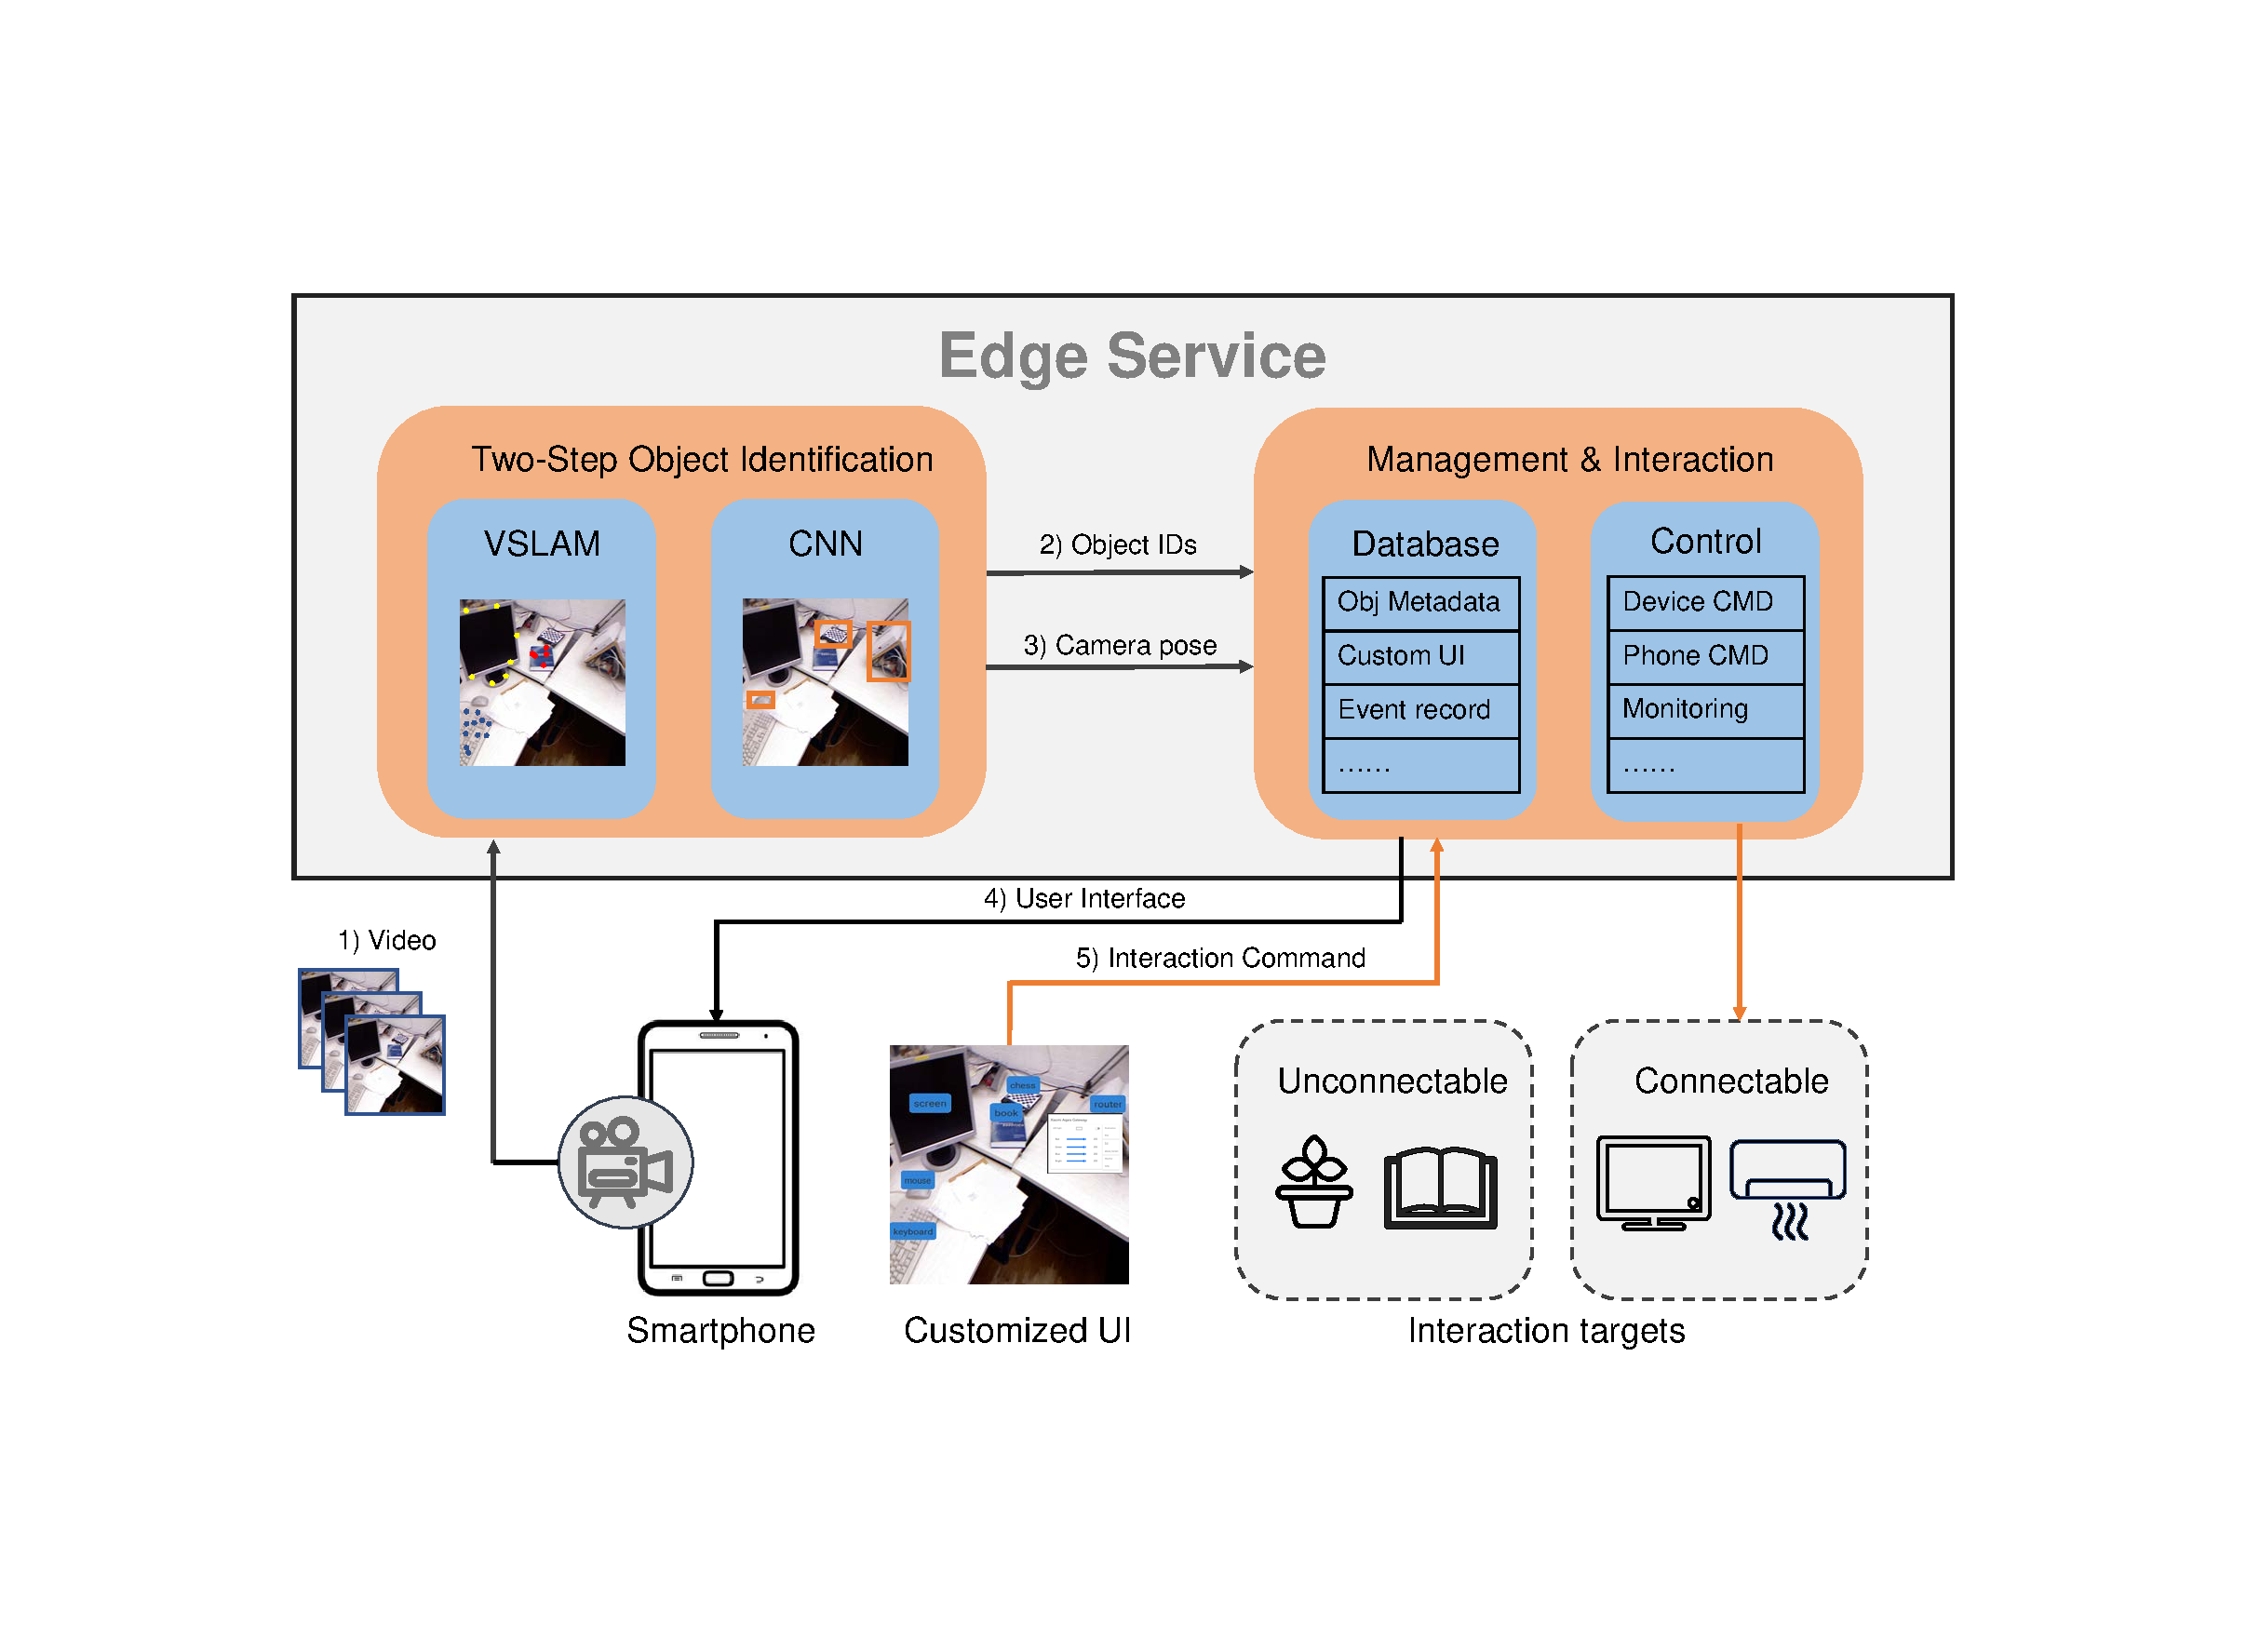
\includegraphics[width=0.99\linewidth]{overview}
	\caption{VSLink总体架构}
	\label{fig:overview}
\end{figure}

\autoref{fig:overview} 显示了我们提出的VSLink的体系结构:来自手机的视频帧被送往边缘服务,边缘服务将对应视频帧中出现的对象UI送回手机端,用户可以使用UI进行交互。在高层次上,交互一共涉及到三端,即手机端、边缘服务端和对象端。我们可以将交互流程总结如下:首先,用户使用智能手机对周围环境进行实时视频拍摄,视频流通过无线链路发送到边缘服务端;第二,边缘服务识别视频帧中的对象,相应的用户界面(UI)及其位置将被发送到智能手机;第三,手机在视频中对象的对应位置处显示UI,用户通过操作UI输入交互命令;最后,该命令由对象/手机/边缘服务根据具体的命令属内容进行处理。

为了实现上述流程并实现用户体验的准确性、速度和质量的目标,在边缘服务端我们提出了两个模块,即两阶段目标识别模块和对象管理与交互模块。目标识别模块识别当前帧中的对象,并在较低的延迟内返回其ID和物理位置。该模块借鉴Visual SLAM和目标检测神经网络的功能,实现快速准确的目标识别。具体来说,我们提前构建了环境的对象级SLAM地图。每次启动VSLink时,边缘服务端都会执行一个Visual SLAM线程。在通过构建的地图定位Visual SLAM的过程中,我们可以使用视觉特征点描述符匹配来识别位置稳定(即相对背景不动)的对象。此外,为了处理移动目标,我们采用了目标检测神经网络。VSLink将Visual SLAM识别结果作为先验,提出了一种基于稀疏卷积的方法,避免了冗余计算。一旦一个物体被神经网络检测到,我们就使用图像检索方法来识别它的ID。

对象管理与交互模块实现了实际的人机交互操作。如果用户命令是由对象执行的,它会将用户命令发送给对象。例如,命令是打开某个设备。为了转发命令,边缘服务端与这些可连接对象建立连接,并集成它们的API。对于不可连接的对象,VSLink也提供了实现交互的功能,这主要依赖于智能手机的功能。

\chapter{两阶段目标识别}
\label{chap:fast}
% \section{动机}
% \label{sec:motivation}
\begin{table}[htbp]
  % \small 
    \centering
    \caption{\label{table:methods}现有目标识别解决方案的可行性}
    \begin{tabular}{|l|l|l|l|l|l|l|}\hline
    方法 &
      分类 &
      ID &
      多目标 &
      移动 &
      环境改变 &
      速度 \\
      \hline 图像分类\cite{he2019bag} &
      {\color[HTML]{355421} √} &
      {\color[HTML]{BF0000} ×} &
      {\color[HTML]{BF0000} ×} &
      {\color[HTML]{355421} √} &
      {\color[HTML]{355421} √} &
      {\color[HTML]{355421} 快} \\ \hline
    目标检测\cite{zou2019object} &
      {\color[HTML]{355421} √} &
      {\color[HTML]{BF0000} ×} &
      {\color[HTML]{355421} √} &
      {\color[HTML]{355421} √} &
      {\color[HTML]{355421} √} &
      {\color[HTML]{BF0000} 慢} \\ \hline
    图像检索\cite{philbin2008lost,zheng2017sift} &
      {\color[HTML]{BF0000} ×} &
      {\color[HTML]{355421} √} &
      {\color[HTML]{BF0000} ×} &
      {\color[HTML]{355421} √} &
      {\color[HTML]{355421} √} &
      {\color[HTML]{355421} 快} \\ \hline
    检测+检索 &
      {\color[HTML]{355421} √} &
      {\color[HTML]{355421} √} &
      {\color[HTML]{355421} √} &
      {\color[HTML]{355421} √} &
      {\color[HTML]{355421} √} &
      {\color[HTML]{BF0000} 慢} \\ \hline
    图像定位\cite{sattler2011fast} &
      {\color[HTML]{BF0000} ×} &
      {\color[HTML]{355421} √} &
      {\color[HTML]{355421} √} &
      {\color[HTML]{BF0000} ×} &
      {\color[HTML]{BF0000} ×} &
      {\color[HTML]{BF0000} 慢} \\ \hline
    Visual SLAM\cite{liu2021edgesharing} &
      {\color[HTML]{BF0000} ×} &
      {\color[HTML]{355421} √} &
      {\color[HTML]{355421} √} &
      {\color[HTML]{BF0000} ×} &
      {\color[HTML]{BF0000} ×} &
      {\color[HTML]{355421} 快} \\ \hline
    \end{tabular}
  \end{table}

在计算机视觉领域,识别图像/视频中感兴趣的目标已经得到了很好的研究。例如,图像分类\cite{he2019bag}、目标检测\cite{zou2019object}、图像检索\cite{philbin2008lost,zheng2017sift}和图像定位\cite{sattler2011fast}可以实现不同程度的目标识别。在\autoref{table:methods}中,我们列出了这些方法的特点,但它们都不符合第\ref{chap:introduction}章中提到的要求。因此,我们将“目标检测+图像检索”方法与Visual SLAM相结合,以实现我们的目标识别。我们之所以选择这两种方法,是因为它们在许多方面表现出互补性。我们可以把环境中的物体大致分为两类,稳定的和可移动的。稳定物体往往位于固定位置,例如电视和空调。可移动的通常从一个地方移动到另一个地方。“对象检测+图像检索”方法(为了简化表示,我们在下面省略图像检索)能够识别所有对象,但由于需要经过神经网络运算,所以速度较慢,而Visual SLAM可以识别稳定对象且速度较快。

\begin{figure}[htb]
  \centering
  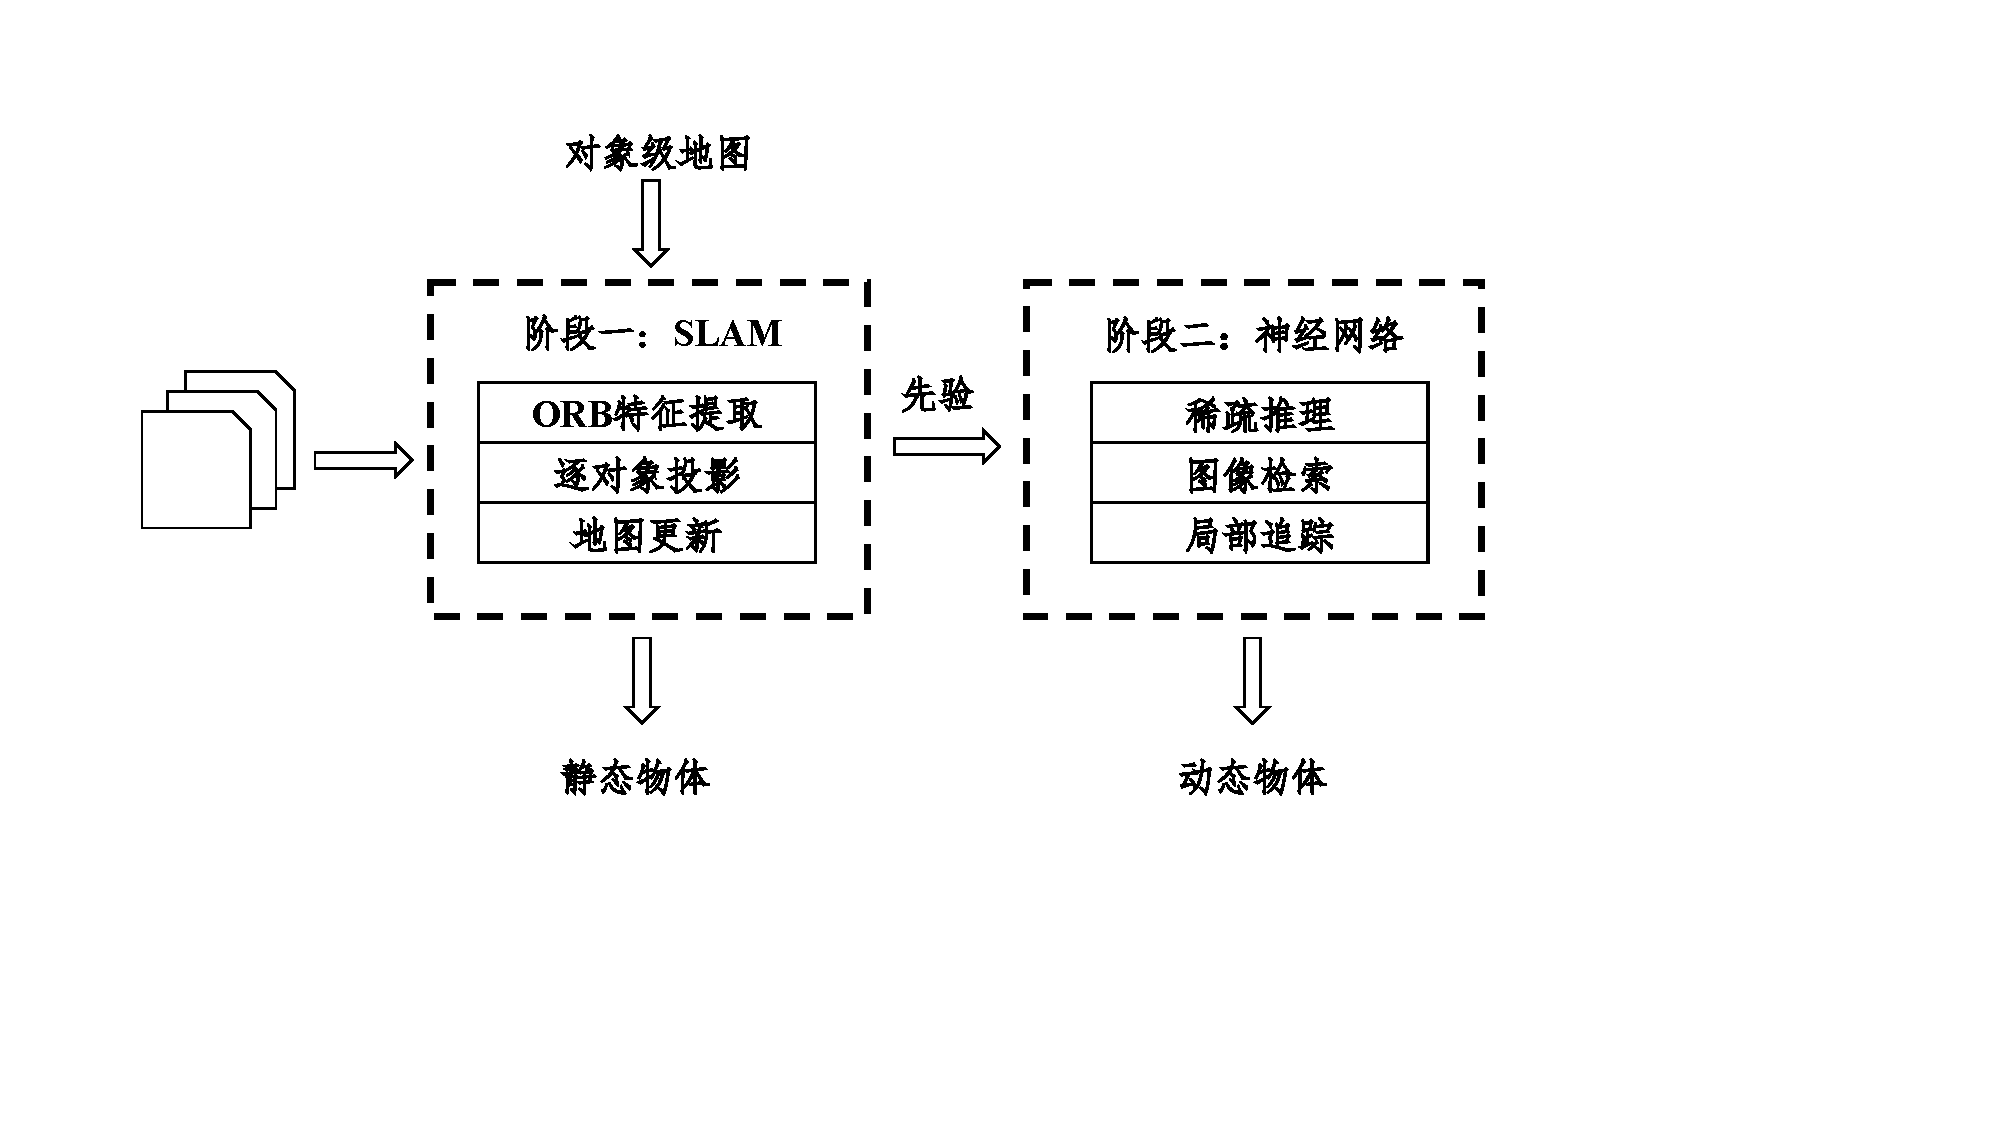
\includegraphics[width=0.75\linewidth]{two-step}
  \caption{两阶段目标识别方法框架}
  \label{fig:two-step-workflow}
\end{figure}

\autoref{fig:two-step-workflow}显示了所提出的两阶段目标识别方法的框架。这种设计接近于实际人脑的工作方式。例如,如果一个人进入卧室,她/他可以立即知道电视的位置,并对自己进行基本定位。然而,要识别手机,他需要集中注意力搜索。因此从直觉上来说,我们可以利用Visual SLAM的空间感知快速识别稳定的对象,然后让神经网络处理可能发生移动的对象。同时,神经网络不需要对整个图像进行分析,只需要对SLAM未识别的区域进行分析,可以大大减少时间开销。




   
\section{基于Visual SLAM的目标识别}
\label{sec:vslam}
SLAM被认为是实现更真实AR体验的关键技术之一,因为它提供了对环境的理解和跟踪。在VSLink中,我们建立了一个终身对象级SLAM地图,这有利于SLAM跟踪和对象识别。

我们选择Visual SLAM来帮助识别对象的原因是:
1) Visual SLAM本身就是为实时视频中的定位而设计的,延迟低;
2) 在SLAM过程中提取的视觉特征,有助于识别可见物体;
3) Visual SLAM提供了环境理解,因此可以支撑进一步的AR开发。
Visual SLAM的一个典型使用场景是,机器人从原点开始其旅程,并在定位自身的同时构建环境地图。
而VSLink与之略为不同,我们将构建一个对象级的三维地图并将其存储在{\edg}中,然后智能手机可以使用该地图定位自身。
% 通常,Visual SLAM可以包括在图像定位类别中,因为它们

\subsection{工作流程}
在这里,我们解释了所提出的基于Visual SLAM的对象识别解决方案的理论。由于经典的Visual SLAM\cite{mur2017orb,engel2014lsd}技术试图在机器人第一次进入环境时实现精确的地图和定位,我们想知道机器人第二次进入环境时是否能够识别它所看到的物体。

\begin{figure}[htb]
  \centering
  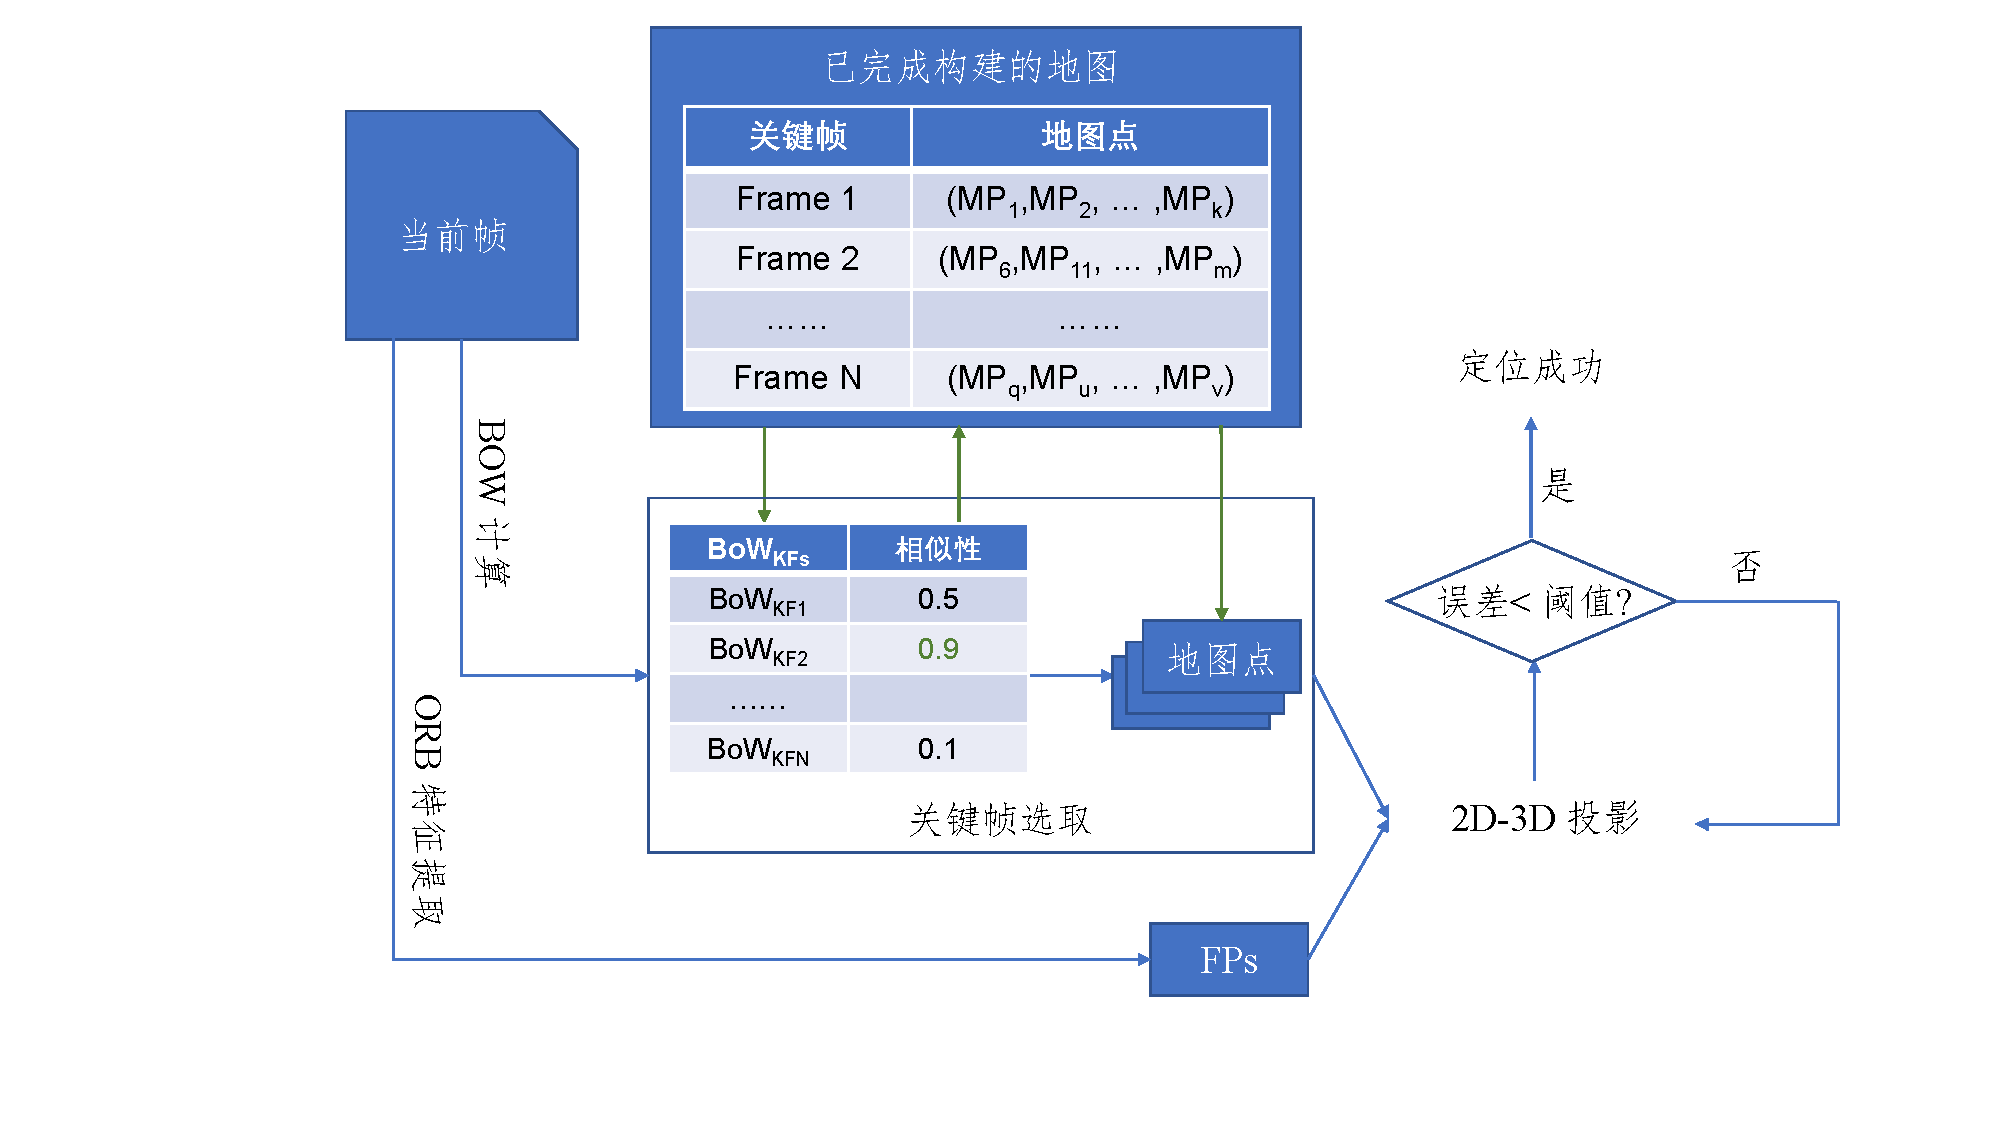
\includegraphics[width=0.8\linewidth]{workflow}
  \caption{ORB-SLAM\cite{mur2017orb}在地图重用时的定位过程}
  \label{fig:localization}
\end{figure}

构建的SLAM地图\cite{mur2017orb}仅包括某些地图点和关键帧,地图重用过程如\autoref{fig:localization}所示。定位过程首先使用单词包(Bag of Words, BoW)\cite{galvez2012bags}计算当前帧的表示,然后计算当前帧和关键帧之间的BoW相似性。然后,它选择具有高相似性的关键帧作为候选帧。最后,对于每个选定的关键帧,它使用RANSAC\cite{derpanis2010overview}算法计算当前帧中的特征点与该关键帧的贴图点之间的2D-3D投影。如果投影误差小于阈值,则定位完成。

我们注意到,上述过程的实质是在地图点$mp = [x_m,y_m,z_m,\vec{orb}]$(在重用的地图中)和特征点$fp = [x_f,y_f,\vec{orb}]$(在当前框架中)之间建立投影,其中下标$m$和$f$表示地图坐标系和框架坐标系。
因此,如果我们给$mp$一个表示对象ID的标签,并且在定位期间将该$mp$投影到某个$fp$,则相应的对象将在当前帧中完成定位。
与原始Visual SLAM相比,在标记贴图点后,我们能够在不引入额外计算的情况下识别环境中的对象。
需要注意的是,此方法不只是记住对象的位置,当对象相对于其在地图上的位置移动时,可能会导致误检测。
ORB特征用于建立2D-3D投影,这意味着SLAM在环境中定位自身后,当某些特征点可见时,它会识别到对象。

虽然不常见,但是我们也考虑了稳定物体移动的情况,我们使用了逐对象投影算法来检测这种运动并更新地图。


\subsection{对象级地图}
\label{sec:map}
为了实现基于Visual SLAM的对象识别,我们需要用相应的对象ID标记地图点。因此,我们称之为对象级地图。

最近,学术界已经开始研究语义SLAM\cite{bowman2017probabilistic,kaneko2018mask}和对象级SLAM~\cite{mccormac2018fusion++,strecke2019fusion}并显示出巨大的潜力。这些工作的典型做法是同时运行SLAM过程和语义分割神经网络,并使用分割结果来细化构建的地图。

\begin{figure}[htb]
	\centering
	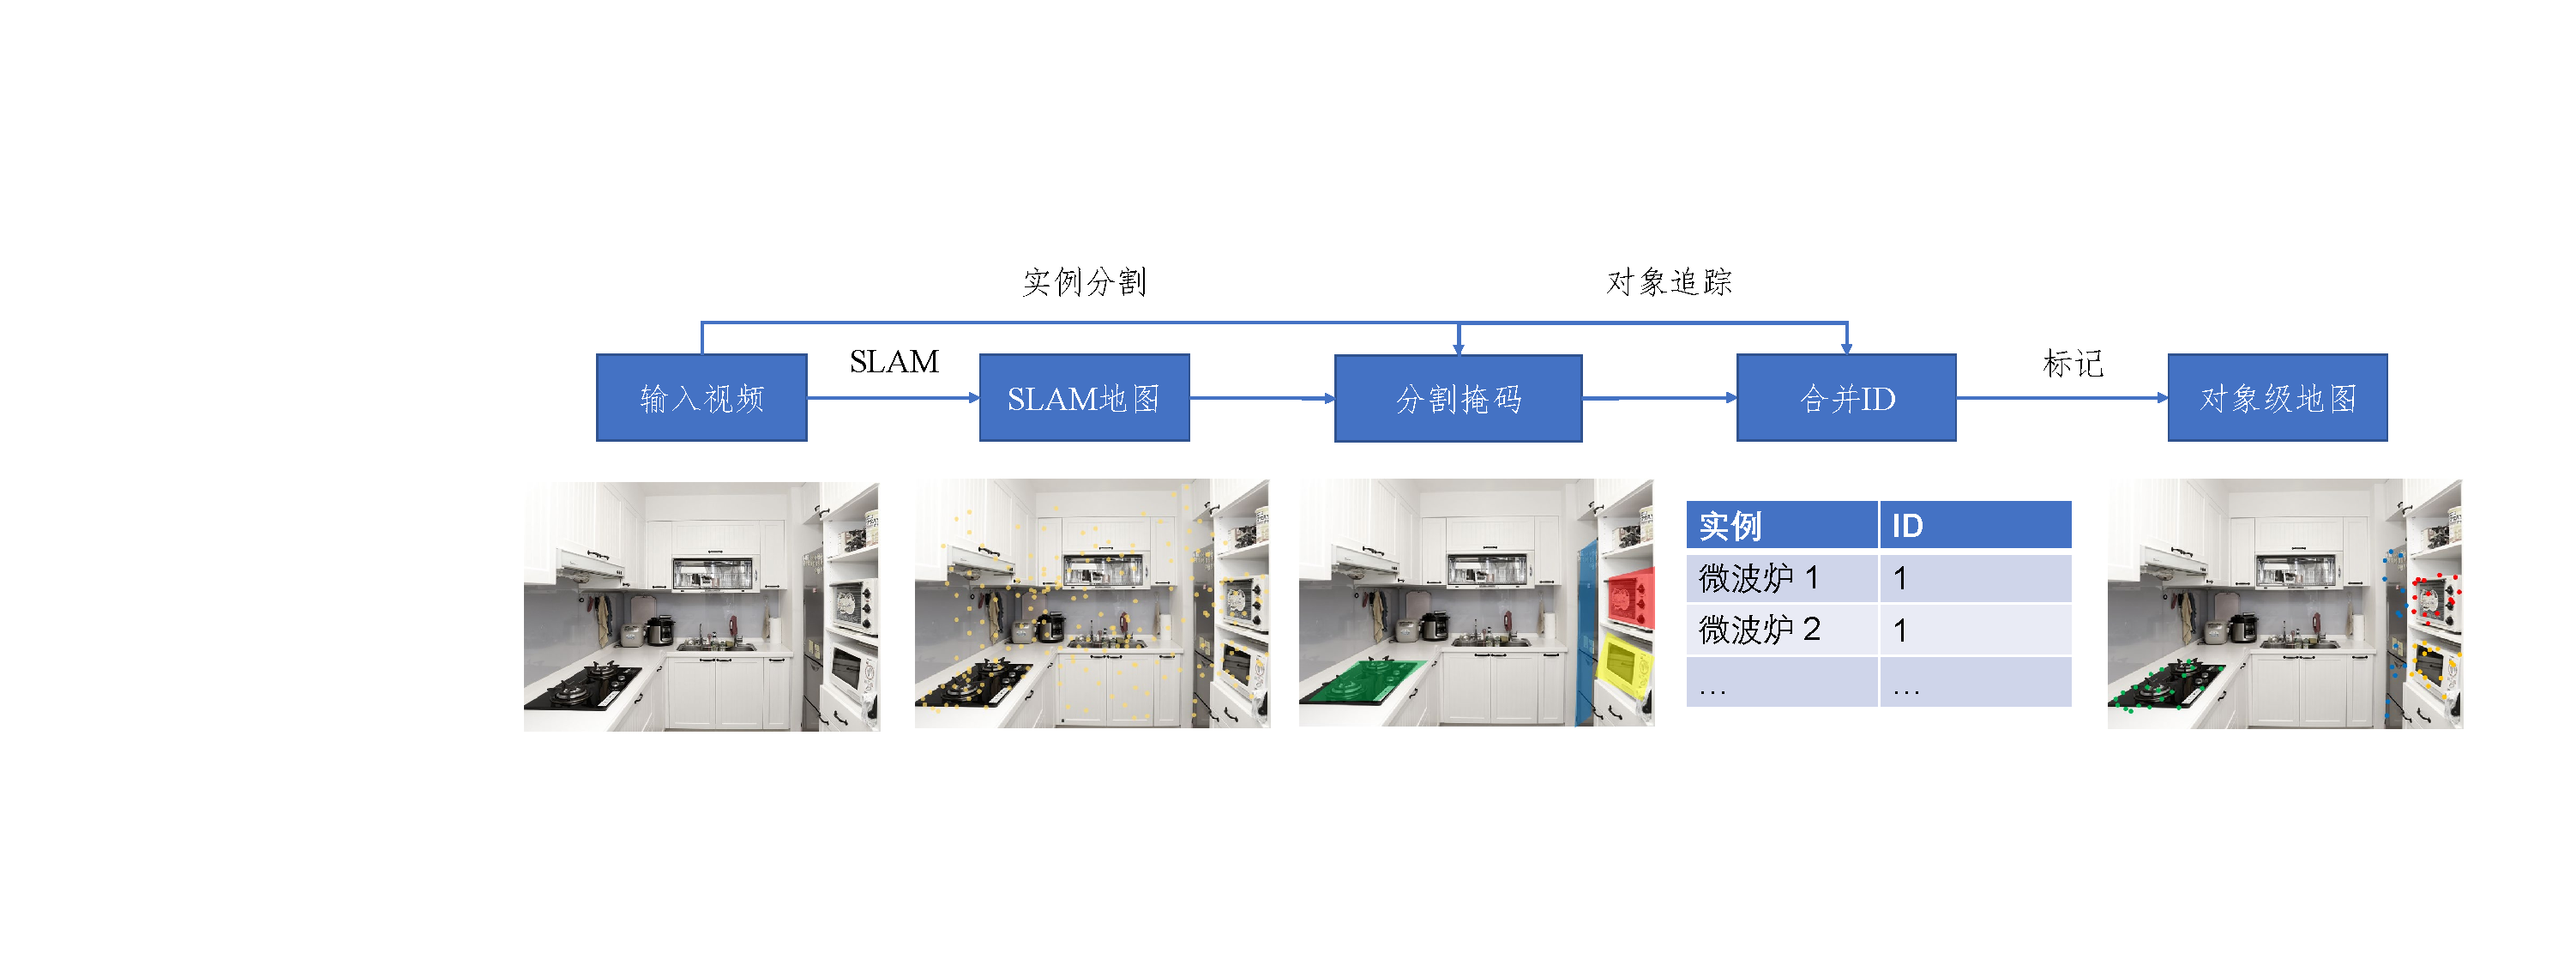
\includegraphics[width=0.99\linewidth]{offline-map}
	\caption{对象级地图的构建过程}
	\label{fig:offlinemap}
\end{figure}

\autoref{fig:offlinemap} 演示了构建对象级地图的工作流。
首先,我们将视频输入原始Visual SLAM进程~\cite{mur2017orb},并构建包含关键帧和地图点的地图。
我们想要确定 1)环境中的哪些对象可以被视为交互目标,2)对于每个地图点,它链接到哪个对象。
因此,我们使用实例分割神经网络\cite{He_2017_ICCV}来实现对输入视频的分割。对于每个检测到的对象,分割结果是像素级的二进制掩码$m$和对象类别$c$。
现在,我们在连续的帧中获得了很多对象,但它们还没有唯一地分配ID。为了防止潜在的重复检测,我们采用对象跟踪神经网络在不同的帧中合并相同的对象。
检测到的对象和地图点之间的链接是像素坐标。
在SLAM过程中,当关键帧中的地图点可见时,我们记录其像素坐标$(x,y)$,整个记录为$\{Index_m,Index_{kf}, (x,y)\}$。
对于每个关键帧的每个地图点,我们检查它们的坐标。如果坐标位于该关键帧的对象掩码内,则使用相应的对象ID标记地图点。
整个过程只需要很少的人工工作量,即拍摄视频并为已识别的对象提供实例标签。

\subsection{地图长期重用}
在建立上述地图之后,我们可以使用该地图来识别稳定的对象。
如果稳定物体永远保持在同一位置,上述方法可以很好地工作。
然而,这在实践中很难实现。
如果稳定对象的位置与地图中记录的位置相比发生变化,我们希望主动检测此类变化并更新地图,从而使地图能够长期使用。

这里我们介绍计算2D-3D投影的RANSAC\cite{derpanis2010overview}算法,并观察移动的对象如何影响该算法。
选择具有类似BoW表示的候选关键帧后,RANSAC计算每个属于关键帧的$mp$和属于当前帧的$fp$之间的ORB特征相似性$s(ORB_{mp}, ORB_{fp})$。如果$s$低于某个阈值,$mp$和$fp$就会成功匹配,这意味着它们属于同一个物理点。
现在,RANSAC将随机选择$n$对匹配项,并通过PnP解算器计算投影$T$
\begin{equation}\label{equ:pnp}
    T = PnP([mp_1, fp_1],[mp_2, fp_2], ..., [mp_n, fp_n]).
\end{equation} 

然后,用$T$检查其余匹配点对,
\begin{equation}\label{equ:check}
    \
    err = T \cdot [mp_x, mp_y, mp_z] - [fp_x, fp_y],
\end{equation} 
其中下标$x,y$和$z$表示$mp/fp$的坐标。
当误差小于阈值时,这对点被视为一个内点,否则它是一个离群点。
在找到足够的内点后,$T$被视为正确的投影,并且将基于所有内点计算新的$T$。相反,如果没有找到足够的内点,RANSAC将从随机选取$n$对匹配项并从第一步开始重新启动。
因此,如果对象移动,潜在的结果可能是1)没有足够的内点进行定位,2)内点包含属于移动对象的地图点,从而导致错误的定位和识别。

我们修改了RANSAC算法,通过计算逐对象的投影来处理这样的对象移动。
在执行PnP解算器以计算$T$之前,我们根据地图点的对象标签对其进行聚类。
我们使用基于背景$T_{background}$的投影作为基准,因为背景通常是稳定的。
对于每个对象$O_i$,我们使用属于$O_i$的可见地图点来验证$T$:

\begin{equation}\label{equ:gdt}
\
err = \Sigma \ T \cdot [mp_x, mp_y, mp_z] - [fp_x, fp_y].
\end{equation}
如果误差高于阈值,这意味着该对象的异常值太多,则我们确定该对象已移动。
详细的算法在算法\ref{alg::poa}中描述。
可以通过投影粗略地估计移动,因此我们仍然可以在正确的位置显示交互UI。
为了实现长期重用,我们需要根据\ref{sec:map}节发送这些视频帧来更新地图。

\begin{figure}[htb]
	\centering
	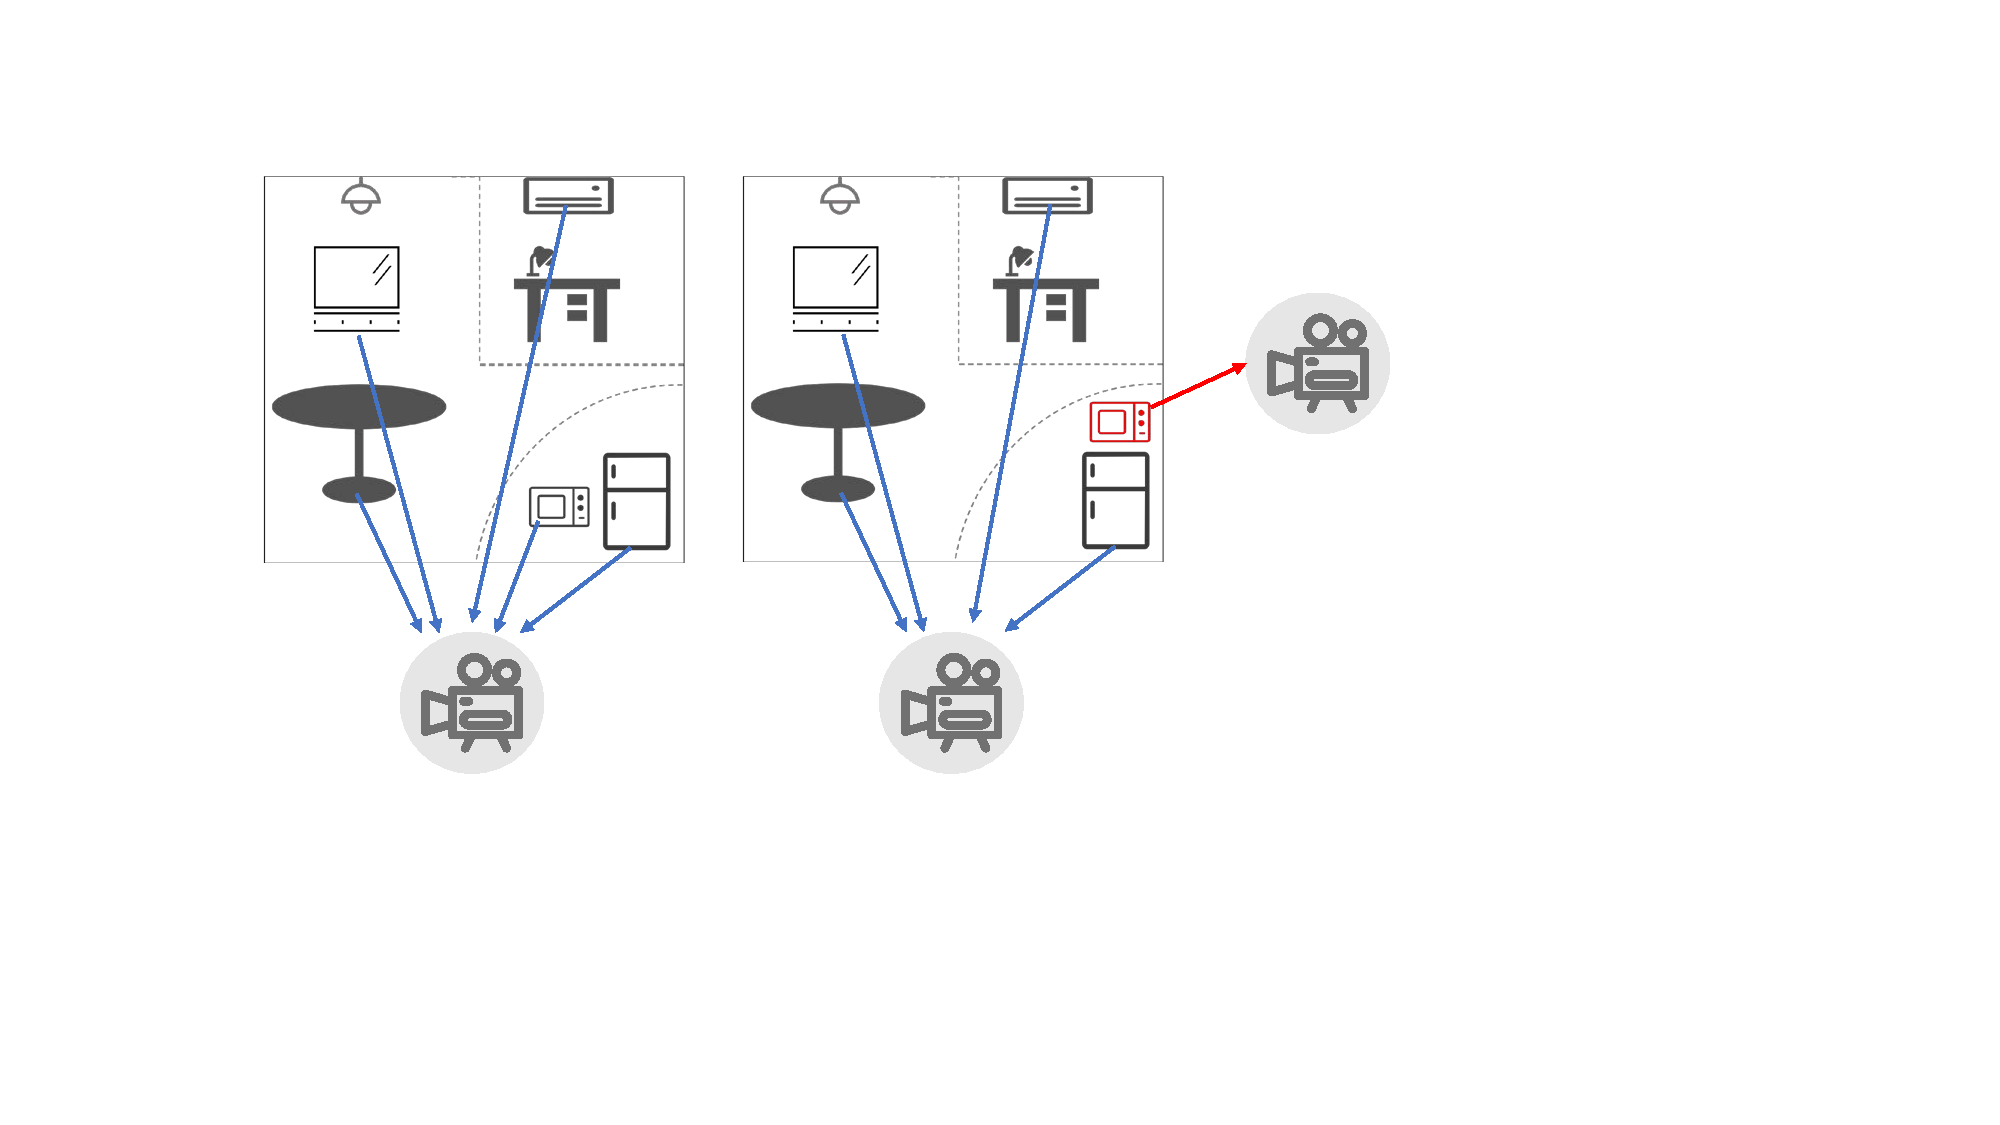
\includegraphics[width=0.7\linewidth]{moveobj}
	\caption{静态和动态目标的识别}
	\label{fig:move}
\end{figure}

\begin{algorithm}[htb]  
	\caption{逐对象投影算法}  
	\label{alg::poa}  
	\begin{algorithmic}[1]  
		\Require  
		$frame$: current video frame;
		$FPs$: feature points of $frame$;  
		$KFs$: keyframes of the map;  
		$MPs$: map points of the map;
		$OBJs$: q visible objects in $frame$;   
		\Ensure  
		camera pose $T_{cw}$;
		movement of $i_{th}$ object $OM_i$;
		\State initial $OM_i=0, i = 1,2,...,q$;
		\State initial $S_{mp}^i=\varnothing, i=1,2,...,q$;
		\State compute bag of words (bow) feature $bow_f$ for $frame$;
		\State Search $KFs$ for frames that share the same word with $bow_f$, then pick the most similar keyframe $KF_{candi}$;
		\For{each $mp\in KF_{candi}$}
		\For{each $fp\in frame$}
		compute the similarity $sim$ between $mp$ and $fp$;
		\If {if $sim < thre$}
		\State $S_{mp}^i = S_{mp}^i\cup\{(mp,fp)\}, i = mp_{label}$;
		\EndIf
		\EndFor 
		\EndFor
		\State compute camera pose $T_{cw}^{env} = PnPSolve(S_{mp}^i)$, $i$ corresponds to the ID of environment;
		\For{each $obj\in OBJs$}
		\For{each $mp\in S_{mp}^i$,  $i$ corresponds to $obj$ ID}
		\State compute camera pose $T_{cw}^{i} = PnPSolve(S_{mp}^i)$;
		\EndFor
		\EndFor
		\State compute and delete outlier in ${T_{cw}^{i}, i=1,2,...,q}$;
		\State recompute camera pose $T_{cw}$ with the left $S_{mp}^i$;
		\If {$T_{cw}^{i}$ is  outlier}
		\State $OM_i = Move_{cal}(T_{cw}^{i}, T_{cw})$; 
		\Else 
		\State {$OM_i = \vec 0$};
		\EndIf
	\end{algorithmic}
\end{algorithm}  

\subsection{基于ORB特征的目标识别}

在建立上述地图后,我们可以使用该地图进行非常快速的目标识别。
整个过程与SLAM中的定位流程紧密耦合,因此让我们首先介绍SLAM如何使用现有地图实现定位。
对于基于关键点的SLAM(如ORBSLAM2),它有一个关键帧数据库。
在定位模式下,它将计算当前帧的BoW特征,并在关键帧数据库中查找相关单词(Word)。然后,通过比较提取的关键点和地图中的地图点的视觉特征,执行更精确的投影。
将当前帧中的关键点投影到贴图点后,由于地图点已经用ID进行标记,因此可以通过检查标签来识别此帧中存在的对象。

\begin{figure}[htb]
	\centering
	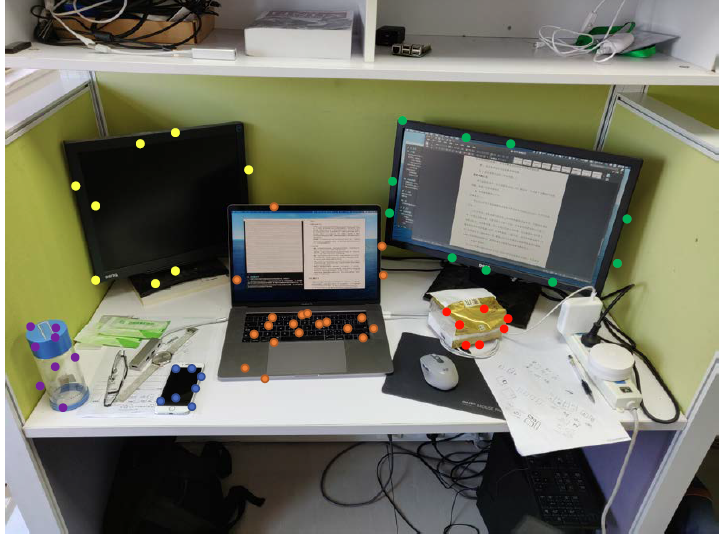
\includegraphics[width=0.75\linewidth]{move3}
	\caption{通过地图点的标签识别对象}
	\label{fig:match}
\end{figure}

\autoref{fig:match}显示了识别结果的示例,通过重新定位识别了五个对象。
请注意,VSLink不使用该位置作为每个对象的定位点,因为对象可以从一个位置移动到另一个位置。在SLAM定位过程中,我们通过视觉特征匹配来检测物体是否存在。


\section{基于稀疏推理的网络加速}
\label{sub:Sparse Object Detection}
在\ref{sec:vslam}节里我们描述了如何利用Visual SLAM和构建的对象级地图来识别稳定对象。然而,我们仍然无法识别会发生位置改变的物体。

如第\ref{chap:fast}章所说,目标识别网络和图像检索可以用于移动物体的识别。目标识别神经网络首先在被检测的物体上产生一个二维的包围盒,然后可以使用图像检索技术在数据库中找到它所对应的ID。

然而这种实现受到神经网络计算时间的限制。尽管研究者们已经在努力通过网络压缩和轻量设计等方式尝试缩短神经网络推理的时间,但在手机上或者只具备CPU的边缘设备上实现实时推理仍然很难做到。


\subsection{检测先验}
% vslam的结果可以产生prior
% mask的产生可以使用前面建图的mask
% 直接依据先验来切分图片的做法结果不好 

我们通过输入约简的方式加快网络推理的速度。
如\ref{sec:vslam}节所述,Visual SLAM可以检测稳定的对象。因此,神经网络不需要对属于稳定对象的区域进行计算。

我们考虑了用于确定检测优先级的不同方法,即如何确定神经网络应忽略的特定区域。
我们可以使用属于某个稳定对象的地图点集作为先验知识来形成该区域。
然而,这种方法提供的先验知识并不完整。
原因是检测到的地图点没有很好地分布在一个物体之上。
在Visual SLAM定位过程中,只有一部分特征点(当前帧中)可以投影到地图点(地图中),并且分布是随机的。
假设我们检测到$N$特征点属于一台电视机,则$N$特征点可能都集中在电视机的一个角落,因而我们并不能排除电视机的主体部分。
不完整的先验使得神经网络必须分析更多的区域,这意味着无法获得更多加速。
为了获得精确完整的先验知识,我们在\ref{sec:map}节中重用实例分割神经网络生成的对象掩码。检测先验可通过以下公式计算:
\begin{equation}\label{equ:mask}
mask_c^i = Trans(Pose_c,Pose_k)mask_k^i.
\end{equation} 

$mask_c^i$表示当前帧中对象$i$的二进制掩码,这是我们的前一帧$mask_k^i$是对象$i$最相关关键帧中的二进制掩码。$Trans(Pose_c, Pose_k)$计算了当前帧和关键帧之间的摄影机姿势变换。

利用检测先验知识,一种直接的减少输入的方法是将原始帧划分为多个子帧,然后分别对其进行推断。
然而,实验表明,这种实现通常比处理原始帧需要更多的时间。
原因是这种“分而治之”的实现降低了计算的并行性。我们需要在for循环中处理这些子帧。此外,许多小尺寸的子帧无法从现有的GEMM优化方法中获益。

\begin{figure}[htbp]
	\centering
	\begin{subfigure}{.45\linewidth}
		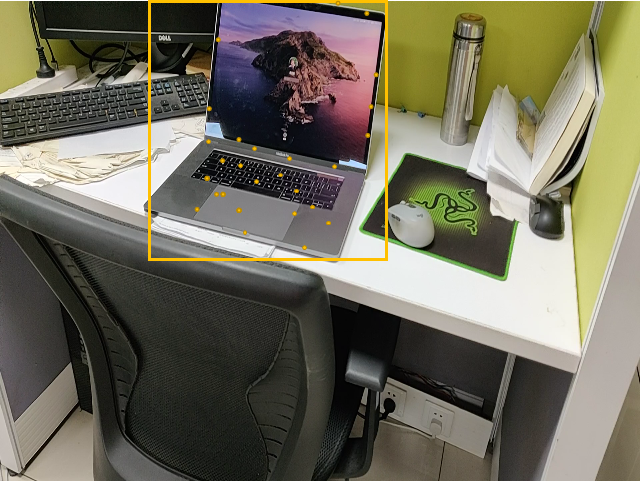
\includegraphics[width=1\linewidth]{sub1-1.PNG}
		\caption{}
	\end{subfigure}
	\ 
	\ 
	\ 
	%\hskip2em\
	%\centering
	\begin{subfigure}{.45\linewidth}
		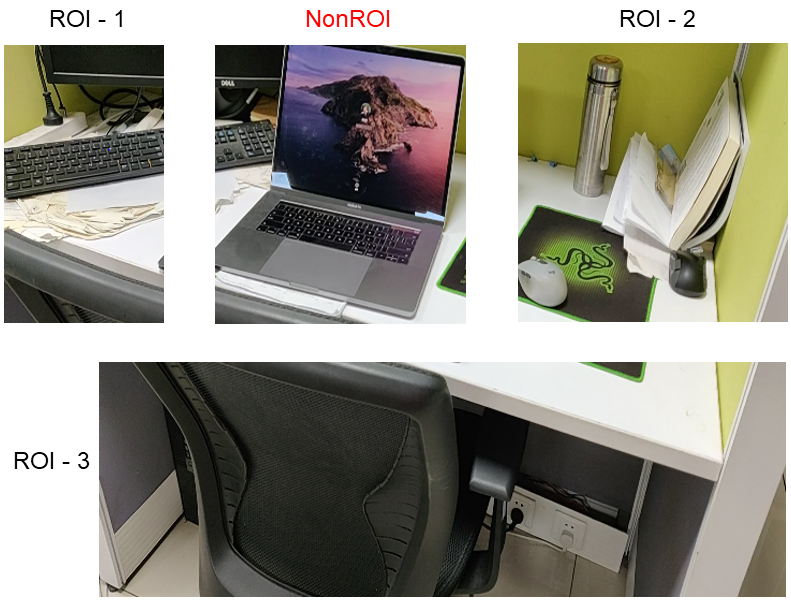
\includegraphics[width=1\linewidth]{sub1-2.PNG}
		\caption{}
	\end{subfigure}
	\caption{使用SLAM的结果产生子图}\label{fig:NN for subgraph}
\end{figure}

\begin{figure}[htb]
	\centering
	\begin{subfigure}{.48\linewidth}
		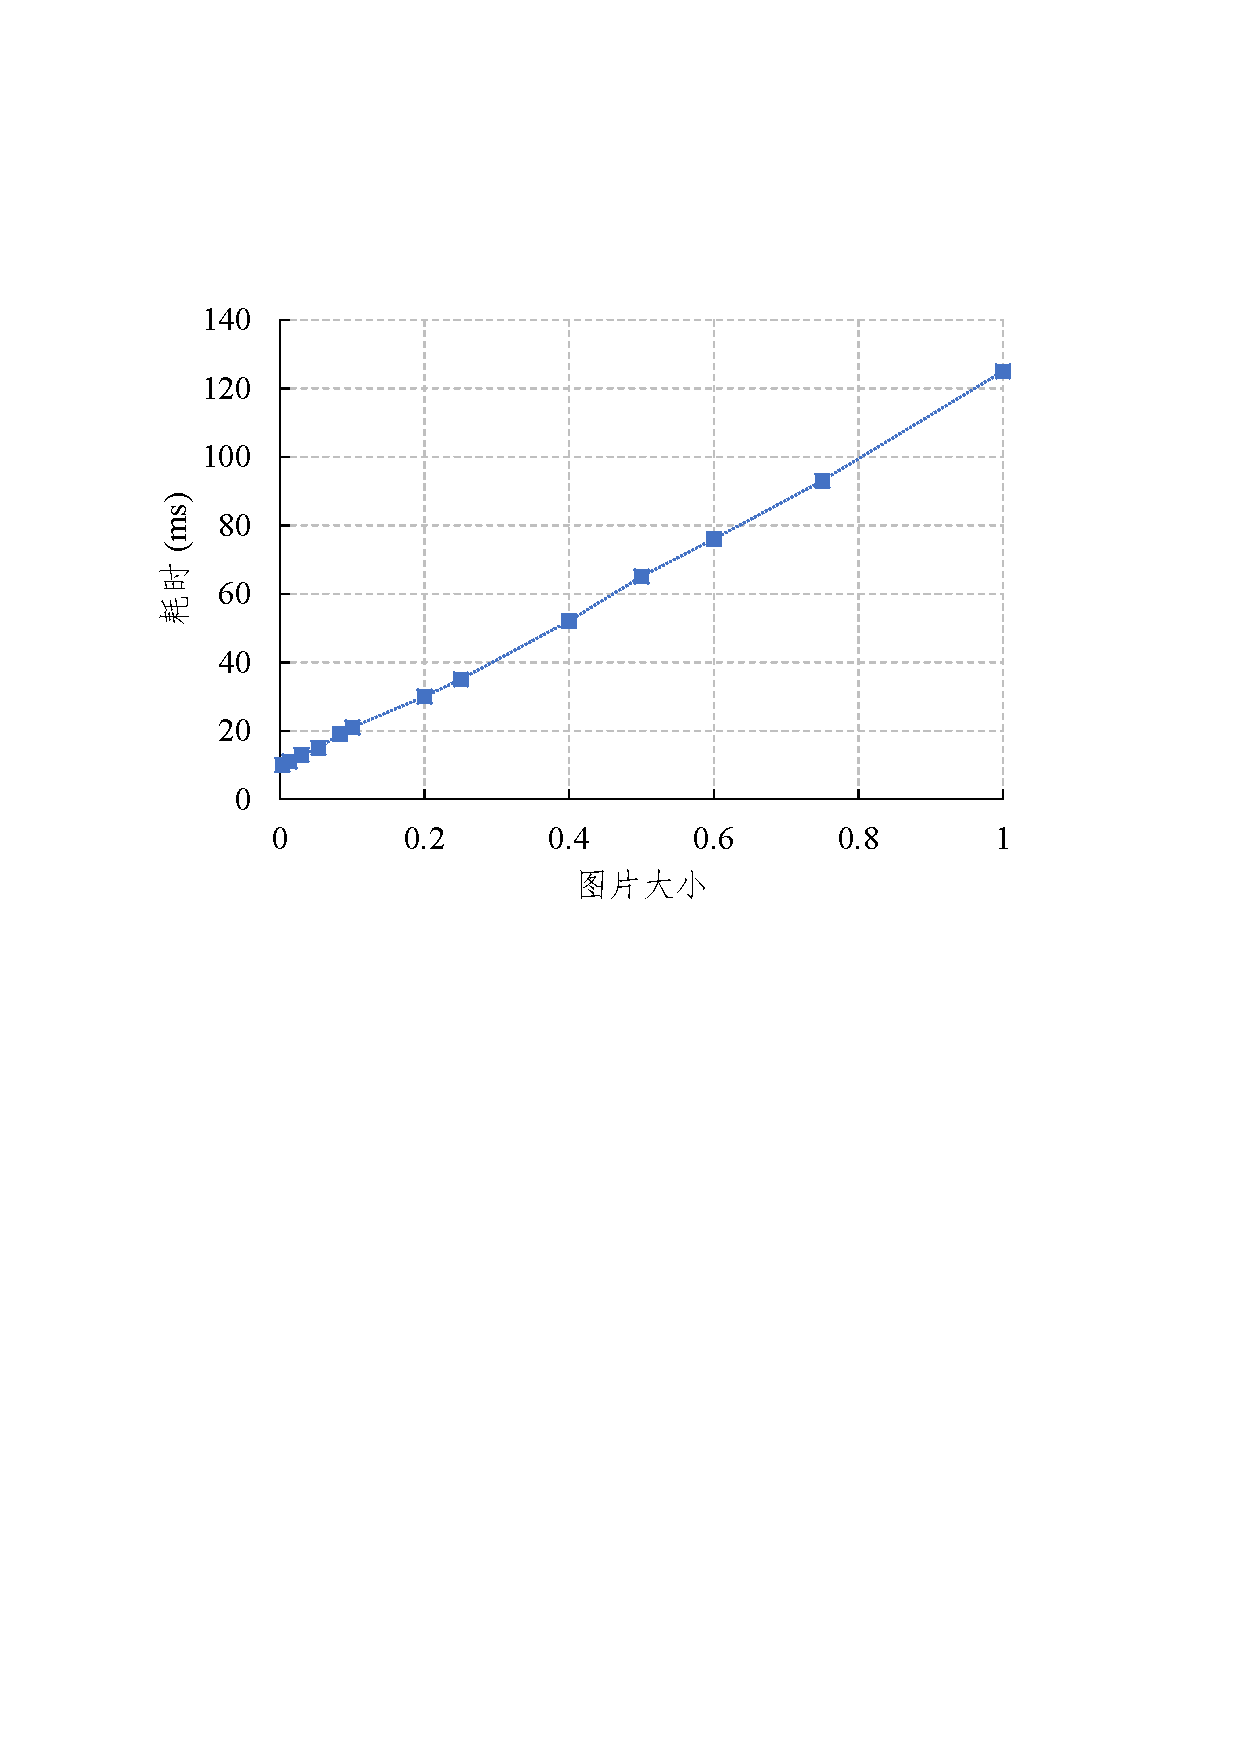
\includegraphics[width=1\linewidth]{static9}
		\caption{}
	\end{subfigure}
	\ 
	%\hskip2em\
	%\centering
	\begin{subfigure}{.48\linewidth}
		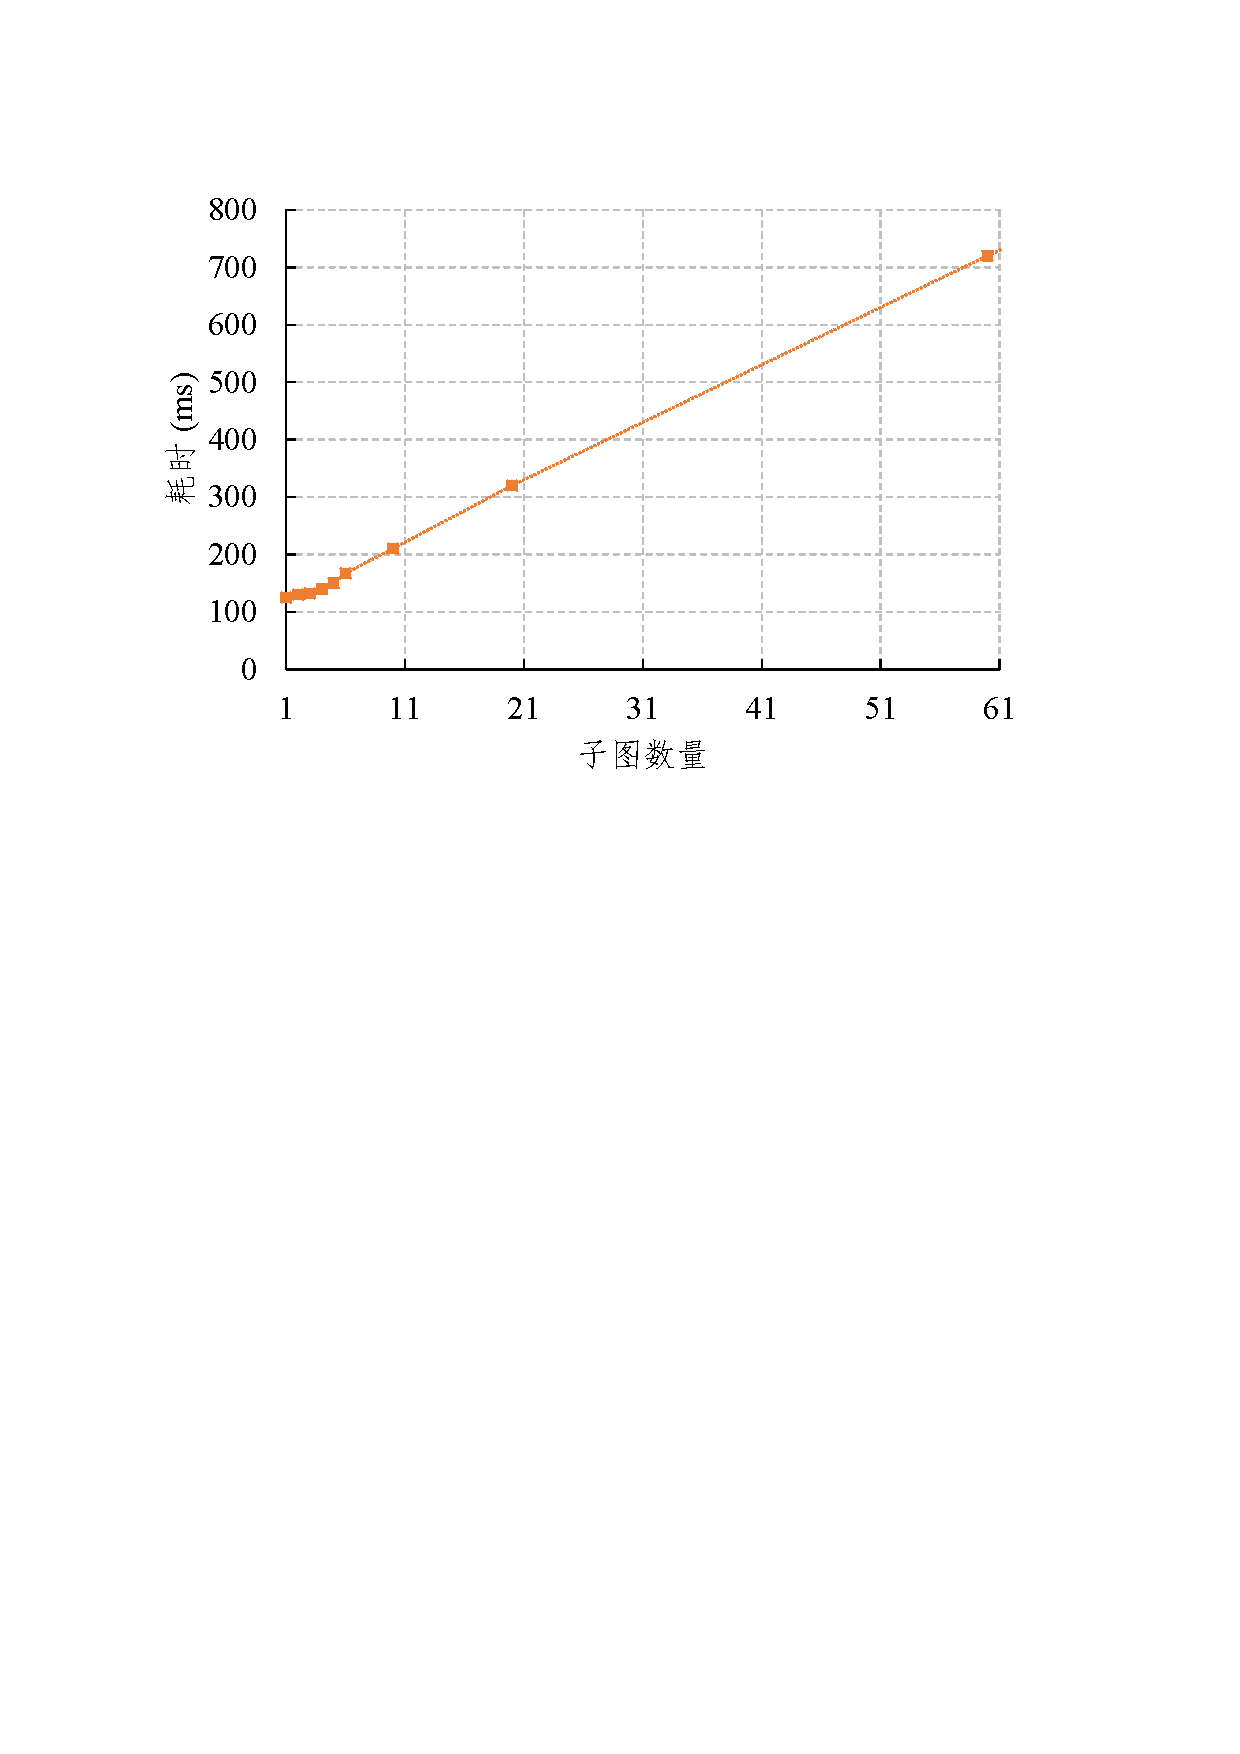
\includegraphics[width=1\linewidth]{static10}
		\caption{}
	\end{subfigure}
	\caption{子图的神经网络推理时间}\label{fig:subframetime}
\end{figure}

从\autoref{fig:subframetime}a中,我们使用$640\times 480$的帧作为标准的图片大小1,图片的大小体现在X轴,我们在不同大小的帧上使用相同的神经网络进行测试,我们可以看到帧的大小$s$和推断时间$t$的关系为$t = as + b, a>0,b >0$,这意味着神经网络推理有一个固定的时间成本,哪怕帧的大小为1个像素点。在我们的测试中,$b$为11毫秒。
\autoref{fig:subframetime}b中,我们将原本的一帧划分成多个子图,测试的结果显示,当我们将帧划分为越来越多的子图时,总的时间开销不断增加。
 
\subsection{稀疏推理}
稀疏卷积\cite{graham2015sparse,ren2018sbnet}可以利用输入的稀疏性来减少延迟。
在VSLink中,我们遵循SBNet\cite{ren2018sbnet}的思想设计了具有稀疏块的目标检测神经网络。

这种稀疏卷积设计~\cite{ren2018sbnet}的关键思想是引入聚集/分散核来实现张量形状变换,只对需要的块进行卷积,以提高运行效率。
基本工作流程如下所示。

首先,我们对需要进行计算的块进行“聚集(Sparse-to-Dense)”操作。
先使用$h\times w$的矩形覆盖原始的像素级二进制掩码,生成一个新的粗粒度的块级掩码。
然后,原始的4维的$N \times H \times W \times C$的帧和2维的$H/h \times W/w$的掩码被发送到卷积块。根据给定掩码中设置为1的$B$个块,利用$h\times w \times C$大小的切片将块从输入张量中切下,并将B个切片沿batch的维度堆叠到新张量中,生成大小为$B\times h \times w \times C$的新张量。

经过聚集操作后,这个新的张量中就只包含我们想要进行计算的部分数据,其余部分则被舍弃,随后我们可以将新张量发送到正常的卷积层进行卷积。

在卷积计算之后,需要对结果进行整形以形成特征图,即“分散(Dense-to-Sparse)”,该特征映射由分散核实现。
分散过程中,我们根据原先使用到的块级掩码将卷积结果的$h\times w \times C$的切片按照原先的位置提取到特征图中。整个推理加速如\autoref{fig:sparse-conv}所示,图中特征图引出的箭头表示下一层会重复类似的计算过程。

\begin{figure}[htb]
	\centering
	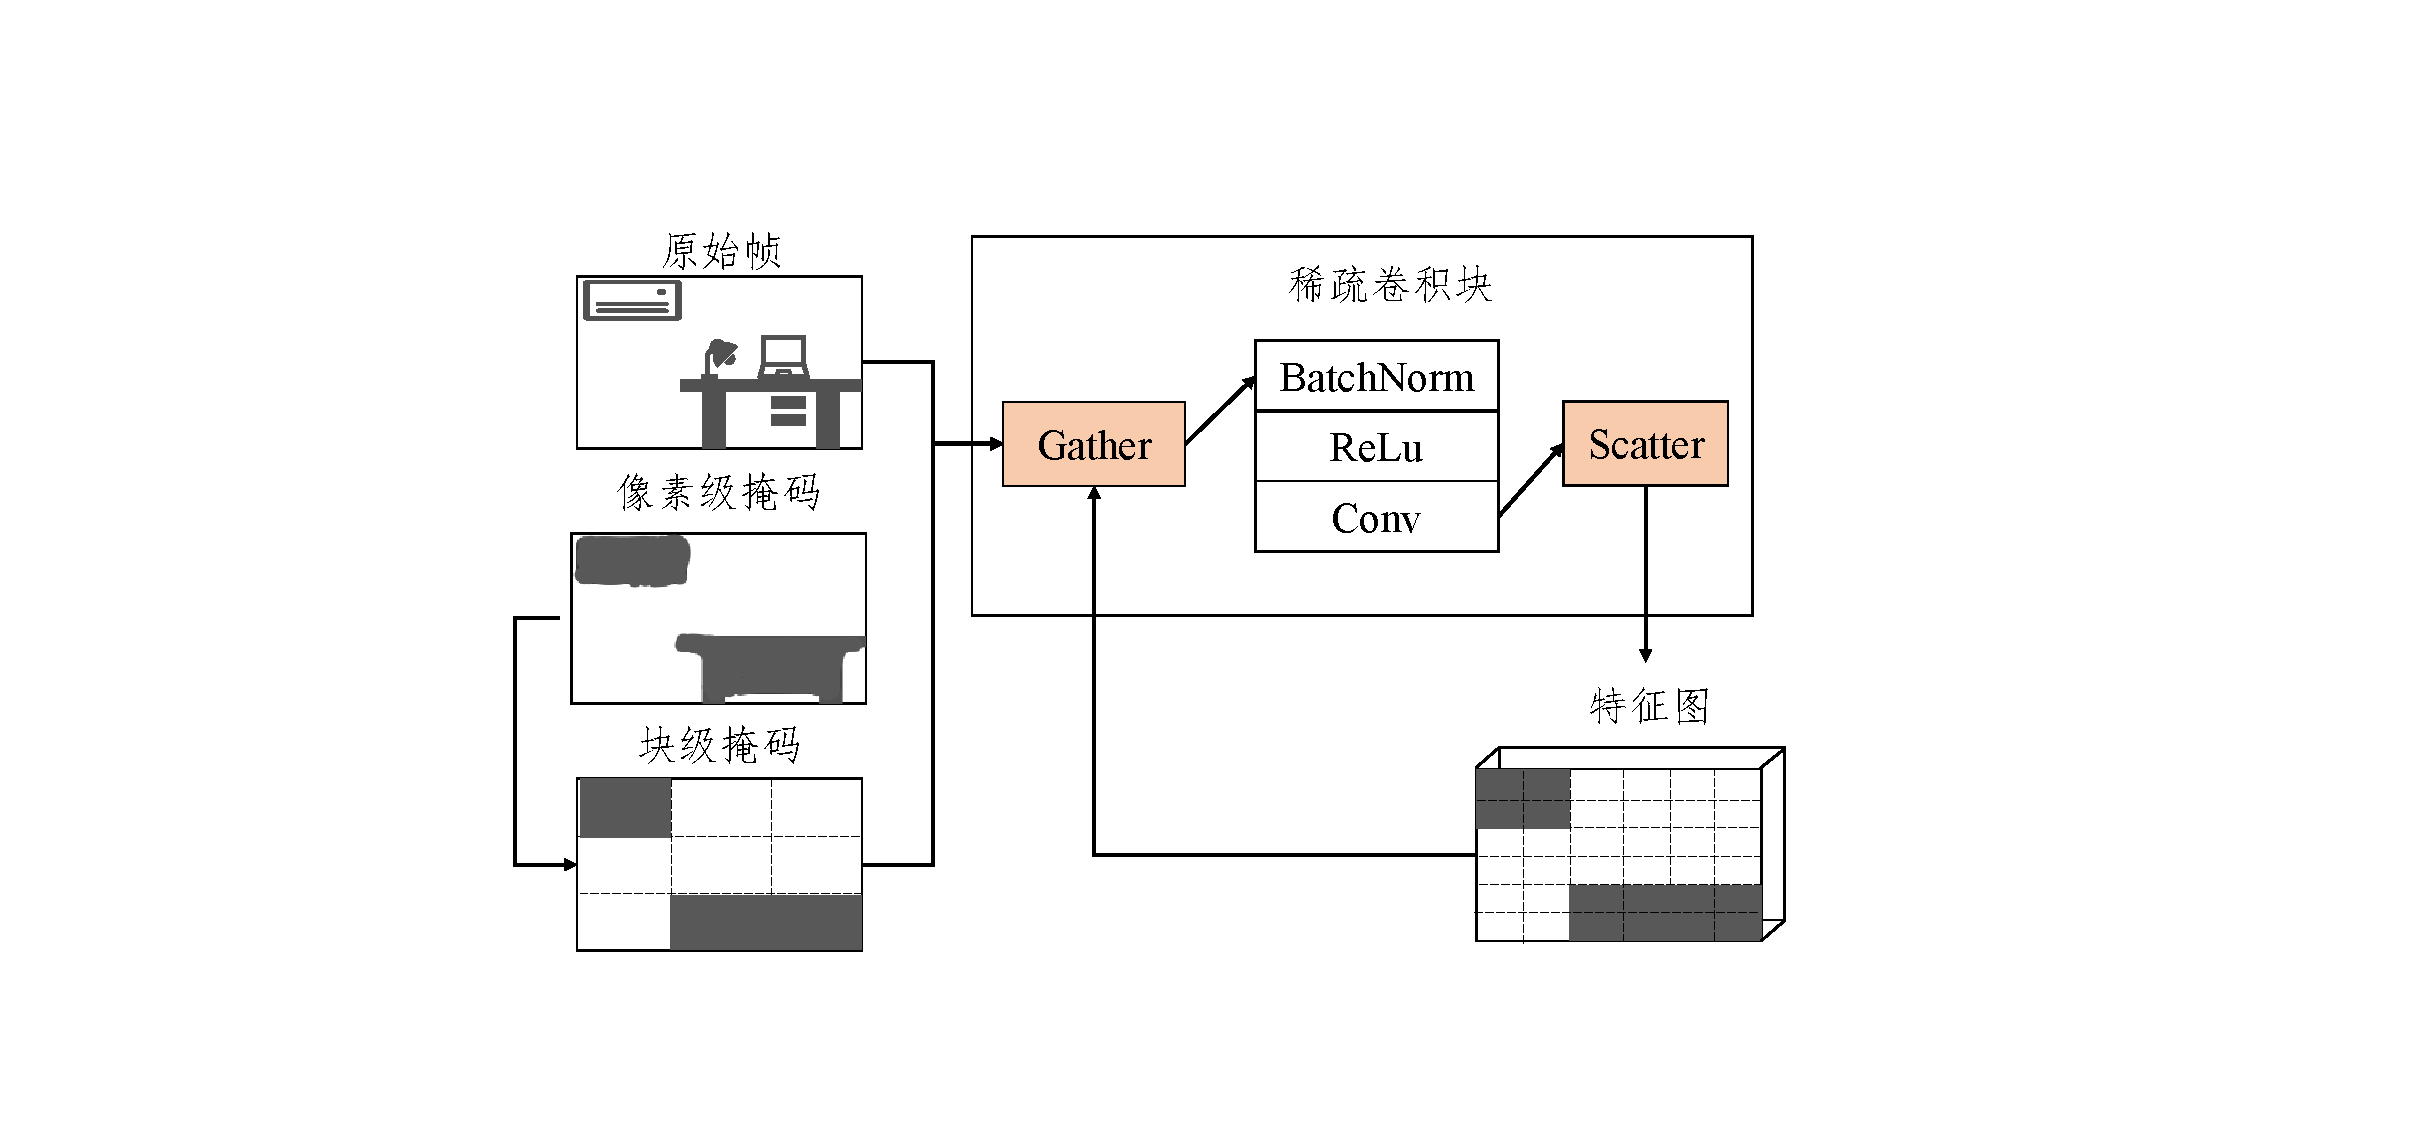
\includegraphics[width=0.75\linewidth]{sparse}
	\caption{推理加速方法工作流程}
	\label{fig:sparse-conv}
\end{figure}

\subsection{识别和追踪}
如果一个物体被神经网络检测到,我们通过图像检索来识别它的物体ID。检索基于的是图像的深度卷积特征。
在构建\ref{sec:map}节所述地图的过程中,我们使用与目标检测神经网络相同的骨干网络提取并保存检测到的可移动目标的深度卷积特征。
在图像检索过程中,对于每个检测到的对象,我们将其特征与数据库中存储的特征进行比较。如果特征相似性达到一个阈值,我们就可以认为识别到了对象。
运动目标的跟踪是通过特征点跟踪来实现的,与稳定目标的跟踪类似。
只要特征点在连续的帧中可见,我们就临时跟踪属于某个可移动对象的特征点。



% \begin{table}[t]
% 	\centering
% 	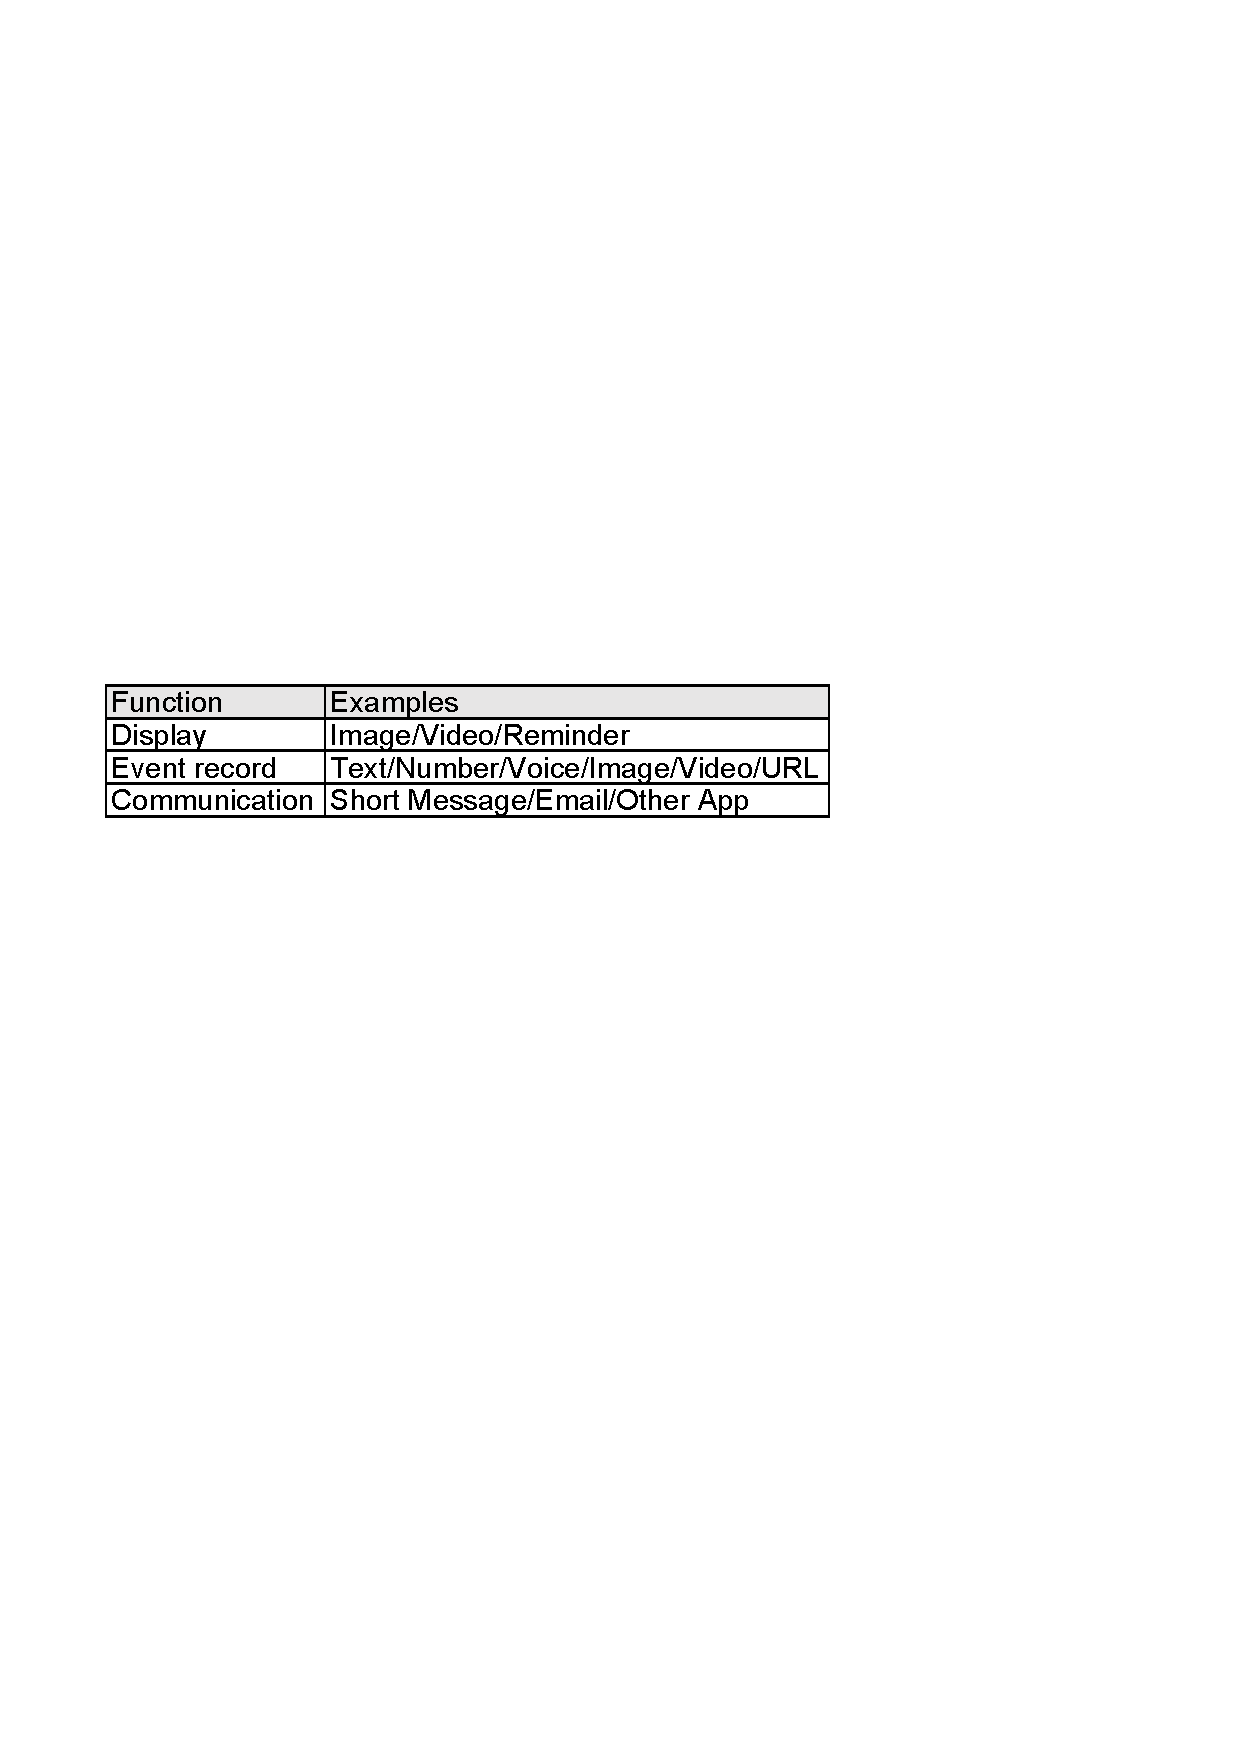
\includegraphics[width=0.98\linewidth]{functions}
% 	\caption{VSLink在不可连接对象上实现的功能}
% 	\label{table:functions}
% \end{table}

\chapter{定制化交互}
\label{chap:flexible}

VSLink旨在丰富人与对象之间的交互。
大多数现有的人机交互实现通常都由程序员决定一切交互行为,比如交互目标、提供的功能和对应的UI。
如第\ref{chap:introduction}章中所述,VSLink通过增加不可连接的对象扩展了交互目标的概念,这意味着用户可以自由确定对象是否为交互目标。由此也带来一个问题,即我们并不知道用户会希望指定什么对象作为交互目标,因此我们需要为此设计对应的机制来解决这个问题。
对此我们的设计理念是让用户决定如何交互,也就是我们提供所有基础功能组件,而让用户决定使用哪些功能组件,并自行设计交互界面。





\section{功能抽象}
为了实现与不同对象的交互,VSLink需要实现相应的UI。
然而,为每个可能的对象设计完整的UI,包括功能和外观,实际上是无法做到的。
即使对象属于同一类别,功能稍有不同也会使得交互方式发生细微改变。
例如,与普通灯相比,智能LED灯具有更多的功能,例如颜色调节和亮度调整。
因此,VSLink提取和抽象对象的\textbf{最小功能单元},并基于这种抽象设计UI。
对于可连接对象,制造商已经定义了最小功能单元,我们只需要遵循其接口。
考虑到不可连接的对象没有预定义的接口,我们提出了三种类型的函数来实现交互。
这些功能基于手机的交互方式,我们认为这有助于人机交互。

\begin{table}[htb]
	% \small  
	\caption{VSLink在可连接对象上实现的功能}  \label{table:functions_2} 
	\begin{center}  
		\begin{tabular}{|m{1cm}<{\centering}|m{6cm}<{\centering}|m{8cm}<{\centering}|}  
			\hline  
			\textbf{功能} & \textbf{案例} &\textbf{具体组件}\\ \hline  
			输入 & 文本/数字/开关/日期 & 按钮/开关/多模式切换按钮/方向控制组合按钮/文本输入/日期时间输入/滚动条/拾色器/文件上传 \\ \hline 
			显示 & 文本/数字/录音/照片/视频/网址 & 列表/表格/视频播放器/音频播放器  \\ \hline
			辅助 & 美化布局/页面跳转 & 页面跳转按钮/分割线/标签/标题 \\ \hline
		\end{tabular}  
	\end{center}  
\end{table}

对于可连接设备,我们开发了\autoref{table:functions_2}中的基本功能单元,主要是为设备的各项功能提供输入输出的载体,其中我们在实践中最常用的是按钮/开关,几乎占到80\%以上,这也容易理解,因为各类设备本身的控制器为了设计方便都大量采用按钮和开关;其次是滚动条,用于调节数值,在空调温度调节和亮度调节等方面比较常用。

由于机械实现的控制器很难进行文本、数字乃至日期的输入,因此文本、数字和日期的输入在原本的设备控制器设计上几乎无法见到,但在一些功能上,用键盘或触屏直接输入文本能极大提升使用体验,比如定时功能通常使用一个按钮进行有限范围内的循环选择,并松开来确定,而时间选择元件可以直接滑动选择任意时间。

由于手机端的特性,我们还实现了一些特殊功能,比如打印机原本必须使用电脑连接才可使用,使用文件上传功能单元后,我们可以直接将手机上接收到的文件进行打印。

最后,为了对界面提供一定的美化和逻辑跳转,我们还提供了页面跳转按钮和各类装饰元素,包括分割线/标签/标题等,以实现页面的分割和二级页面的跳转。

\begin{table}[htb]
	% \small  
	\caption{VSLink在不可连接对象上实现的功能}  \label{table:functions}  
	\begin{center}  
		\begin{tabular}{|l|l|}  
			\hline  
			\textbf{功能} & \textbf{案例} \\ \hline  
			显示 & 照片/视频/备忘录   \\ \hline 
			事件记录 & 文本/数字/录音/照片/视频/网址   \\ \hline 
			通讯 & 短信/邮件/其他应用   \\ \hline  
		\end{tabular}  
	\end{center}  
\end{table}

而对于不可连接对象,我们为为其提供了如\autoref{table:functions}所示三个大类的功能单元:

\begin{itemize}
	\item \textbf{显示类}功能单元用于展示信息,包含文本框、图片框以及视频播放器等功能单元,用这类功能单元我们可以在办公室的一面墙上显示每日新闻和计划等信息,或者作为照片墙展示员工风采等;另外还可以提供例如天气、地图等信息的展示。这些功能单元可以以极低的成本提供类似于投影仪和大屏电视的功能;
	\item \textbf{事件记录类}功能单元用于输入信息,包括数字输入框、文本输入框、按钮等功能单元,用这类功能单元我们可以开发出互动功能,以为植物浇水为例,我们可以用一个按钮为植物更新浇水记录,每次按下按钮,就自动更新植物的浇水时间,结合一个文本的展示,为用户提醒上次浇水的时间。
	\item \textbf{通讯类}功能单元用于实现简单的通信功能,比如在留言墙下放置一个邮件发送单元,即可让来访者输入来访感言/意见反馈之后一键向留言墙的主人发送邮件(以一个提前设置的账户发送),为人与人之间的交流提供便利。
\end{itemize}


 
\section{用户定制的UI}
通过获取一组最小的功能单元,用户可以根据个人需要设计完整的用户界面。
VSLink使用基于Web的UI设计框架,用户可以在其中调整对象UI的外观、布局和逻辑。
整个设计过程没有代码,只需要拖放操作。
为了减少用户在设计UI时的负担,我们鼓励用户从UI模板开始自己的设计。
我们提供多个具有代表性的用户界面模板。根据对象类别,建议用户选择某个模板,开始定制UI设计。

为了使用的方便,用户界面可以在使用时通过解锁按钮进行布局解锁,实现在使用时调整布局,而无须在浏览器中进行再次布局。

\section{定制流程}
接下来以LED灯UI界面的定制流程为例,简单介绍用户如何进行定制:
\paragraph{创建页面}
当某个设备接入设备平台后,可以为设备创建专属的交互页面,并在其上定制该设备的交互组件。
创建页面的具体方式是在网址中指定设备名称:
http://[平台网址]/\#/?obj=[设备名称]\&user=[用户名]

如对LED灯,可以将页面命名为led,用户名为abc,则输入如下网址:
http://[平台网址]/\#/?obj=[led]\&user=[abc]

\begin{figure}[htb]
	\centering
	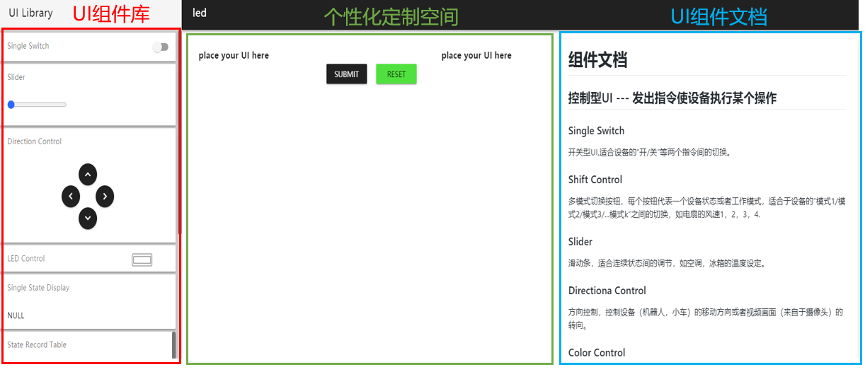
\includegraphics[width=0.95\linewidth]{ui1}
	\caption{新创建的空交互页面}
	\label{fig:ui1}
\end{figure}

访问页面后会提示,是否使用VSLink提供的模板,选择使用模板时会获得一个根据设备名称猜测的界面模板,提前放置了作者设计的简单模板,只需要绑定对应功能即可使用。在选择不使用模板的情况下,我们会得到一个空的交互页面如\autoref{fig:ui1}。页面的左侧是UI组件库,里面显示了所有可用的UI组件;页面右侧是UI组件的文档,可以在文档里查阅每个UI的适用情况;页面中间是UI布局空间,用户可以在这里调整每个UI绑定的对象,以及UI的整体布局。

\paragraph{选取组件}

\begin{figure}[htb]
	\centering
	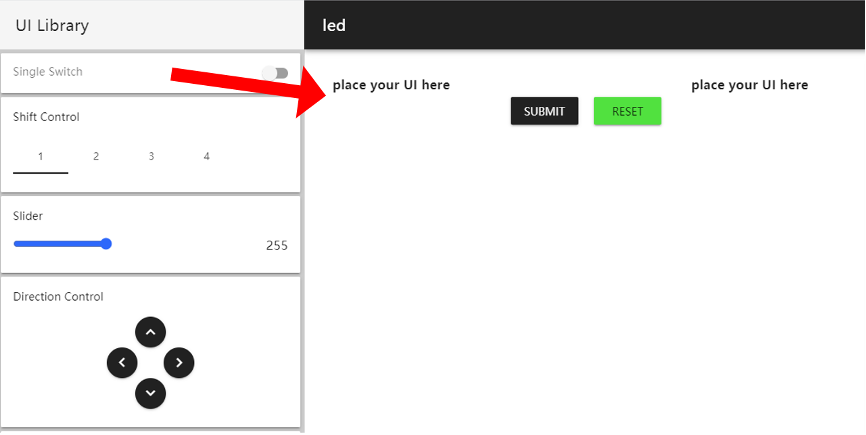
\includegraphics[width=0.65\linewidth]{ui2}
	\caption{拖拽UI组件}
	\label{fig:ui2}
\end{figure}

组件库内包含各类UI组件,我们可以先查看右侧的组件库文档大致了解每个组件的功能。
对于智能LED灯,一般我们会使用到它的四个功能:开关、亮度调节、色彩调节、光照传感器数值查看。

首先选择一个Single Switch组件拖拽至页面中间的个性化定制空间,注意要拖拽到有文字提示”Place your UIs here”的地方。这个组件可以用于LED灯的开关控制。拖拽动作如\autoref{fig:ui2}。如果想删除已经拖拽的UI组件,可以在个性化定制空间单击组件右上方的“-”符号进行删除。

\begin{figure}[t]
	\centering
	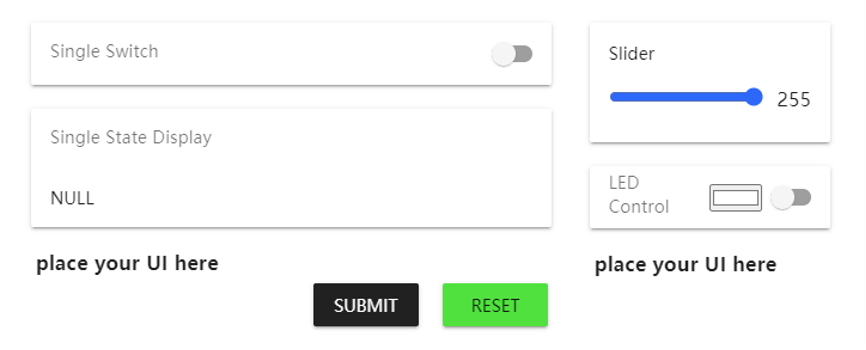
\includegraphics[width=0.65\linewidth]{ui3}
	\caption{UI组件选取结果}
	\label{fig:ui3}
\end{figure}

接着,我们找出Slider组件(控制LED灯亮度)和Color Control组件(用于控制LED灯的色彩),也拖拽到个性化定制空间。用户可能会对室外自然光强度感兴趣,我们也拖拽Single State Display组件,用于显示室外光照传感器的读数。
UI组件选取结果如\autoref{fig:ui3}。

\paragraph{绑定设备}

\begin{figure}[htb]
	\centering
	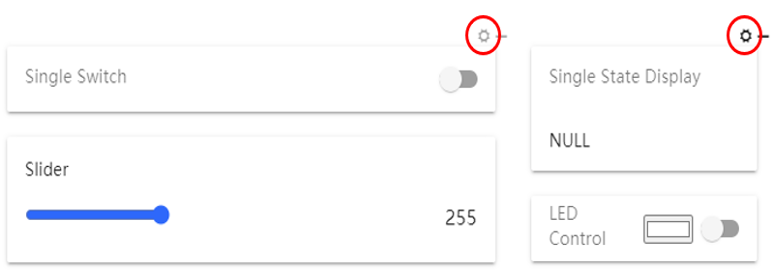
\includegraphics[width=0.65\linewidth]{ui4}
	\caption{新创建的空交互页面}
	\label{fig:ui4}
\end{figure}

按上述步骤选取出来的UI组件,目前并没有对应到真实的设备功能智商,因此我们需要将其与设备的具体功能或属性进行绑定,以激活UI的作用。绑定过程需要在个性化定制空间内完成。首先将鼠标悬停于组件上,组件右上角将出现一个小的设置图标如\autoref{fig:ui4},点击该图标,会弹出组件属性设置对话框。

\begin{figure}[htb]
	\centering
	\begin{subfigure}{.48\linewidth}
		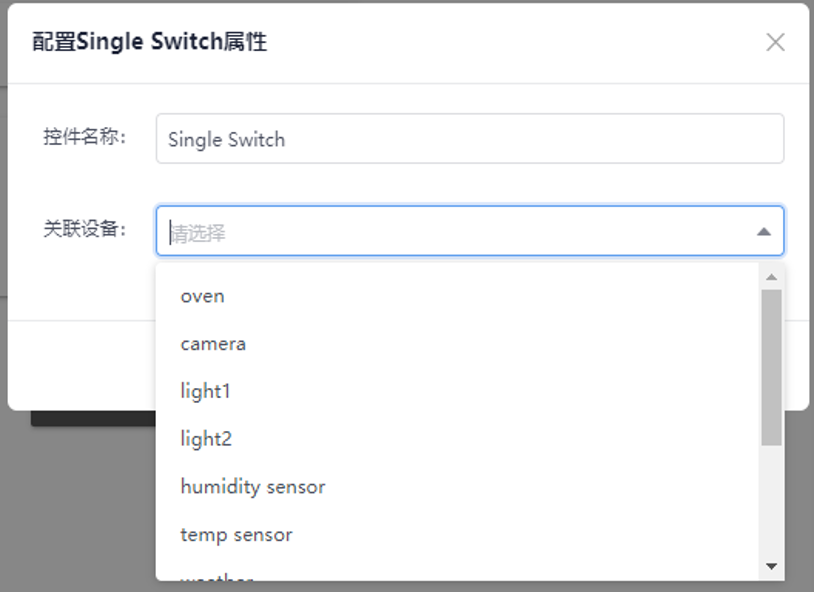
\includegraphics[width=1\linewidth]{ui5}
		\caption{}
	\end{subfigure}
	\ 
	\begin{subfigure}{.44\linewidth}
		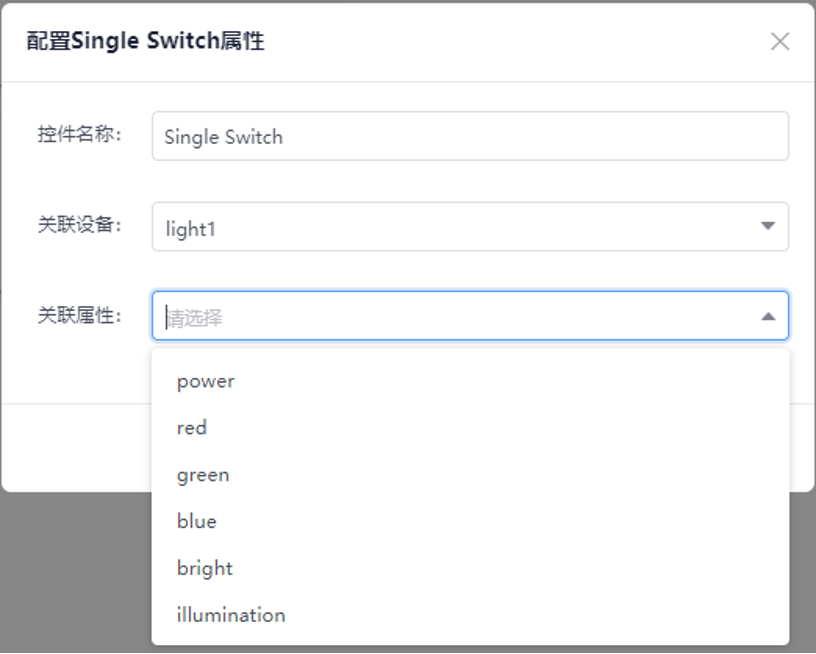
\includegraphics[width=1\linewidth]{ui6}
		\caption{}
	\end{subfigure}
	\caption{为UI关联物理设备和具体功能}\label{fig:ui56}
\end{figure}

如\autoref{fig:ui56}所示,首先将组件绑定的设备选择为light1(即我们将绑定到的真实设备名称),然后我们分别为Single Switch绑定灯的开关,Slider绑定灯的亮度,Color Control绑定灯的色彩。对于Single State Display,我们先为它绑定光照传感器,再绑定传感器读数。

\paragraph{自定义布局}
在上一步,我们完成了UI组件与具体设备功能的绑定。为了有个性化的交互体验,用户可以调整个性化定制空间里的UI布局如\autoref{fig:ui78}。通常会依据使用的方便性和布局美观的标准来调整布局,也就是尽量把使用频率高的组件放在显著的位置,同时整体布局观感良好。我们仍然使用拖拽的方式调整布局。

\begin{figure}[htb]
	\centering
	\begin{subfigure}{.65\linewidth}
		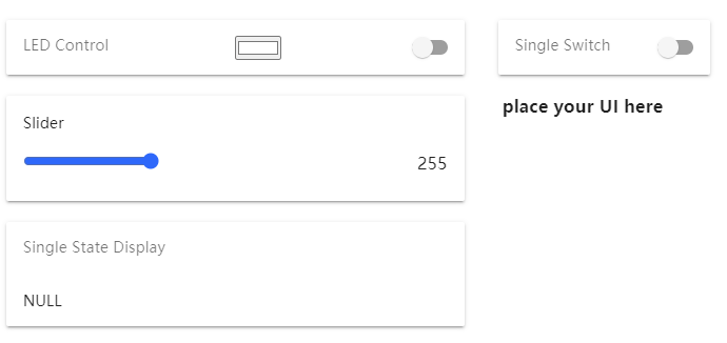
\includegraphics[width=1\linewidth]{ui7}
		\caption{}
	\end{subfigure}
	\ 
	\begin{subfigure}{.65\linewidth}
		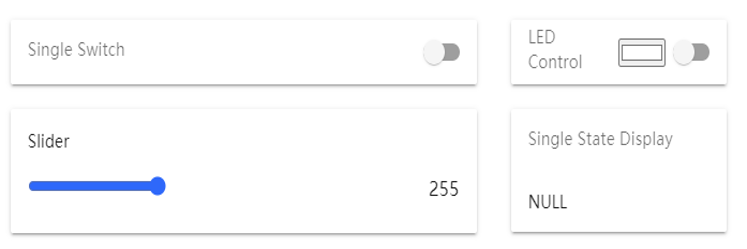
\includegraphics[width=1\linewidth]{ui8}
		\caption{}
	\end{subfigure}
	\caption{布局调整前后}\label{fig:ui78}
\end{figure}

\chapter{实现和验证}
\label{chap:eval}
\section{实现}
\textbf{软件}: 我们基于ORB-SLAM2\cite{mur2017orb}实现了两阶段目标识别模块的Visual SLAM部分,ORB-SLAM2得到了广泛的应用和验证。我们继承了它用于地图构建和跟踪的代码,并开发了地图点标记、对象识别和逐对象投影的代码。
我们在VSLink中采用了SOTA轻量级目标检测模型yolov5s\cite{glenn_jocher_2020_4154370},因为它在速度和准确率上具备优越性。我们修改了网络,使其支持稀疏卷积\cite{ren2018sbnet}。
我们通过LibTorch使得神经网络在C++环境中执行。
对于图像检索,我们使用目标检测神经网络最后一个特征提取层的输出\cite{glenn_jocher_2020_4154370}作为特征表示。两阶段目标识别模块的所有代码都是用C++编写的。

我们为用户实现了一个基于Web的平台,用户可以在其中设计定制的交互。
在前端有基本单元(用于最小功能单元的UI)和画布。
通常,用户可以通过将基本单元拖动到画布来实现自己的设计。
我们还为不同的对象准备了多个UI模板,这可以简化设计过程。
这个平台的代码是用HTML5编写的。
在后端,我们使用HomeAssistant\cite{homeass}作为连接和适配设备的平台,首先在设备接入阶段使用HomeAssistant为各家厂商设备提供的接入方式进行接入,然后在运行阶段利用HomeAssistant对外开放的WebSocket接口获取对应的设备信息并具体设备发出交互命令。

\textbf{硬件}: 我们采用了智能手机Oneplus 7作为移动AR设备,它有一个骁龙855处理器和8GB的RAM。边缘服务端使用一台带有ubuntu系统的PC,它有16G的RAM和一个8核CPU。
\section{实验设置}

我们在真实的校园实验室环境中评估了VSLink。为了收集视频数据,我们在5天内对实验室进行了5次录像。
第一次的视频长度为8分钟,该视频用于构建对象级地图。其余视频的长度为3分钟,用于评估。在第四次和第五次,我们手动更改六个对象的位置。

\section{评估}

\textbf{地图构建}:
在为环境构建地图的过程中,我们首先过滤绑定到非常少地图点的对象。
这是因为地图点的数量直接影响识别性能。在\autoref{table:mps}中我们列出了保留和过滤的对象,我们可以看到过滤后的对象通常尺寸较小或没有丰富的视觉特征,这符合ORB-SLAM2\cite{mur2017orb}的地图点选择方法的原则。
最后,我们选择了20个对象作为交互目标,包括13个可连接对象和7个不可连接对象。

\begin{table}[htb]
	% \small  
	\caption{各类对象所提取的特征点数量(部分)}  \label{table:mps} 
	\begin{center}  
		\begin{tabular}{|l|l|l|l| p{4cm}|}  
			\hline  
			\textbf{被过滤对象} & \textbf{地图点数量} & \textbf{保留的对象} & \textbf{地图点数量}\\ \hline  
			box & 15 & PC & 355  \\ \hline 
			chair & 13 & table & 239  \\ \hline 
			chair & 9 & display & 83  \\ \hline  
			chair & 22 & Paper cutter & 226  \\ \hline  
			box & 43 & printer & 291  \\ \hline  
			chair & 9 & water fountain & 216  \\ \hline  
		\end{tabular}  
	\end{center}  
\end{table} 

\textbf{系统延迟}:
我们将对象识别的VSLink延迟数据与其他方法进行了比较。考虑了两种方法。一种是SnapLink\cite{chen2018snaplink}采用的基于图像定位的方法,另一种是将目标检测神经网络与图像检索相结合。我们用于比较的神经网络是原始的YOLOv5s\cite{glenn_jocher_2020_4154370},没有进行稀疏卷积的修改。

\begin{figure}[htb]
	\centering
	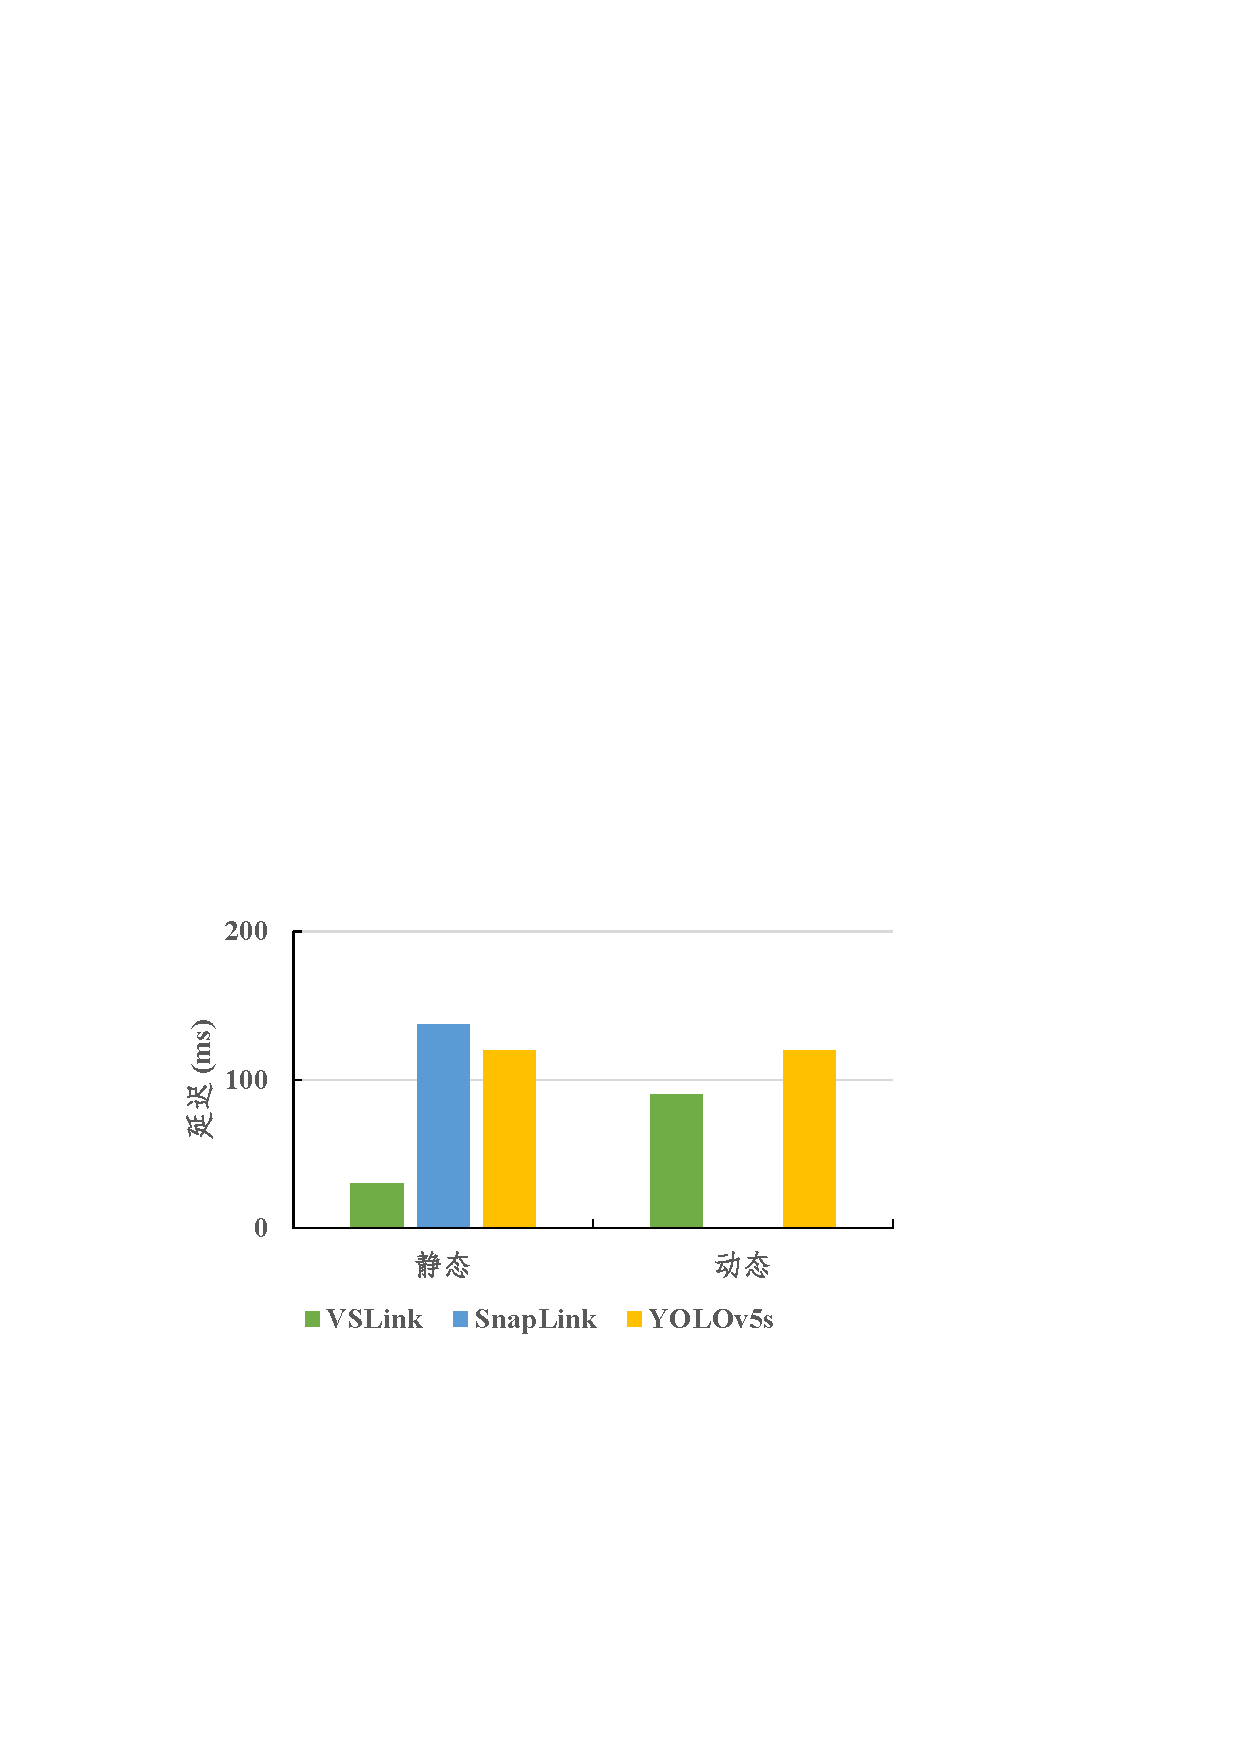
\includegraphics[width=0.65\linewidth]{latency_all.pdf}
	\caption{系统延迟对比}
	\label{fig:latency comparison}
\end{figure}

我们在同一台机器上对四个视频运行了20次这些算法,结果显示在\autoref{fig:latency comparison}中。
首先,我们可以看到,对于那些稳定的对象,VSLink可以在20毫秒内检测到它们的存在,这与ORBSLAM的运行频率一致。在这个过程中,VSLink不需要计算视觉特征,而是重用SLAM结果。
然而,其他两种方法需要更多的时间进行特征计算,即100ms以上。
然后,对于可移动对象,SnapLink无法处理这种情况,因为场景与数据库中的图像不匹配,而对于神经网络,其花费的时间与稳定对象相同,大于100ms。
VSLink平均需要76毫秒左右才能完成加速推理。然而,这不是每个帧都需要的,因为\cite{yao2020video}已经提出了基于帧变化选择性执行对象检测的方法。
因此,VSLink的整个平均处理时间在33ms以下。
虽然原始的YOLOv5s方法不需要等待其他过程,但它完成推断需要120毫秒。
 
总而言之,VSLink可以支持每秒30帧的视频流,用于多对象识别,并且在速度上优于其他两种方法$4$倍。

\begin{figure}[htb]
	\centering
	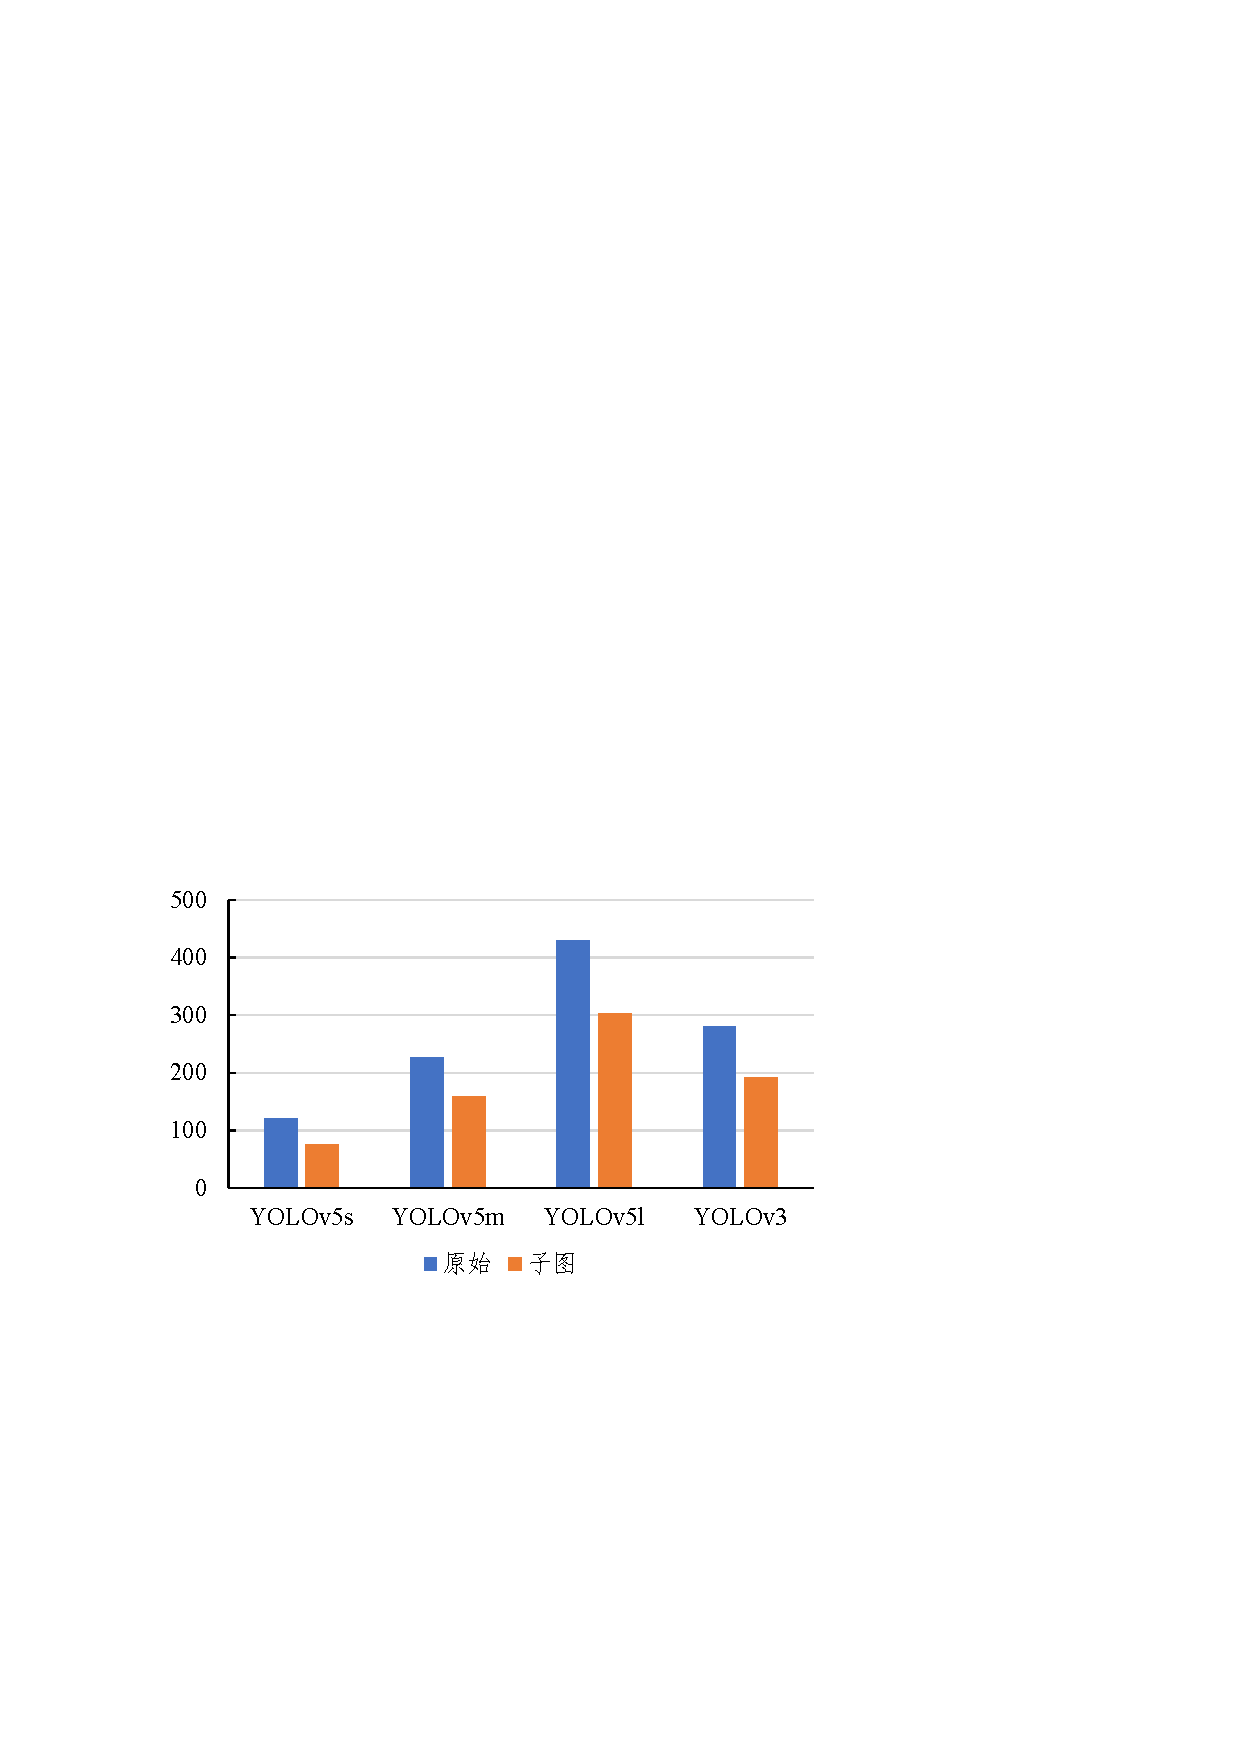
\includegraphics[width=0.65\linewidth]{NN1.pdf}
	\caption{使用子图后目标检测延迟的改善}
	\label{fig:latency improvement}
\end{figure}

\textbf{稀疏推理加速}:
我们采用高性能的目标检测神经网络YOLO\cite{redmon2016you}来评估我们提出的推理加速方法。
我们选择了不同尺寸和结构的模型,分别为YOLOv5s、YOLOv5m、YOLOv5l和YOLOv3,其中s、m、l表示模型尺寸。
所有神经网络都在Pytorch中训练,并使用TorchScript导出。导出之后,可以在C++环境中调用它们。
在\autoref{fig:latency improvement}中,我们通过引入检测先验和稀疏卷积来显示神经网络的延迟减少。这表明所有的神经网络都有延迟下降。YOLOv5s、YOLOv5m和YOLOv5L的速度提升分别为33.1\%、34.4\%和37.0\%。
我们认为更大的模型会得到更好的速度提升。

在实验中,我们对YOLO系列模型进行了测试。
然而,这只是目标检测神经网络的一种类型。
我们认为,只要网络中包含卷积块,理论上所有的目标检测神经网络都将受益于这种推理加速。对于其他类型的神经网络,加速程度将有所不同。
例如,已知更快的RCNN是精确的两阶段模型,加速的过程不同于一阶段模型。
对于两阶段模型,将首先使用RPN生成包围盒,然后使用分类模型生成对象标签。由于涉及到完全连接层,我们需要在一阶段之后进行计算修改。


\begin{figure*}[htb]
	\centering
	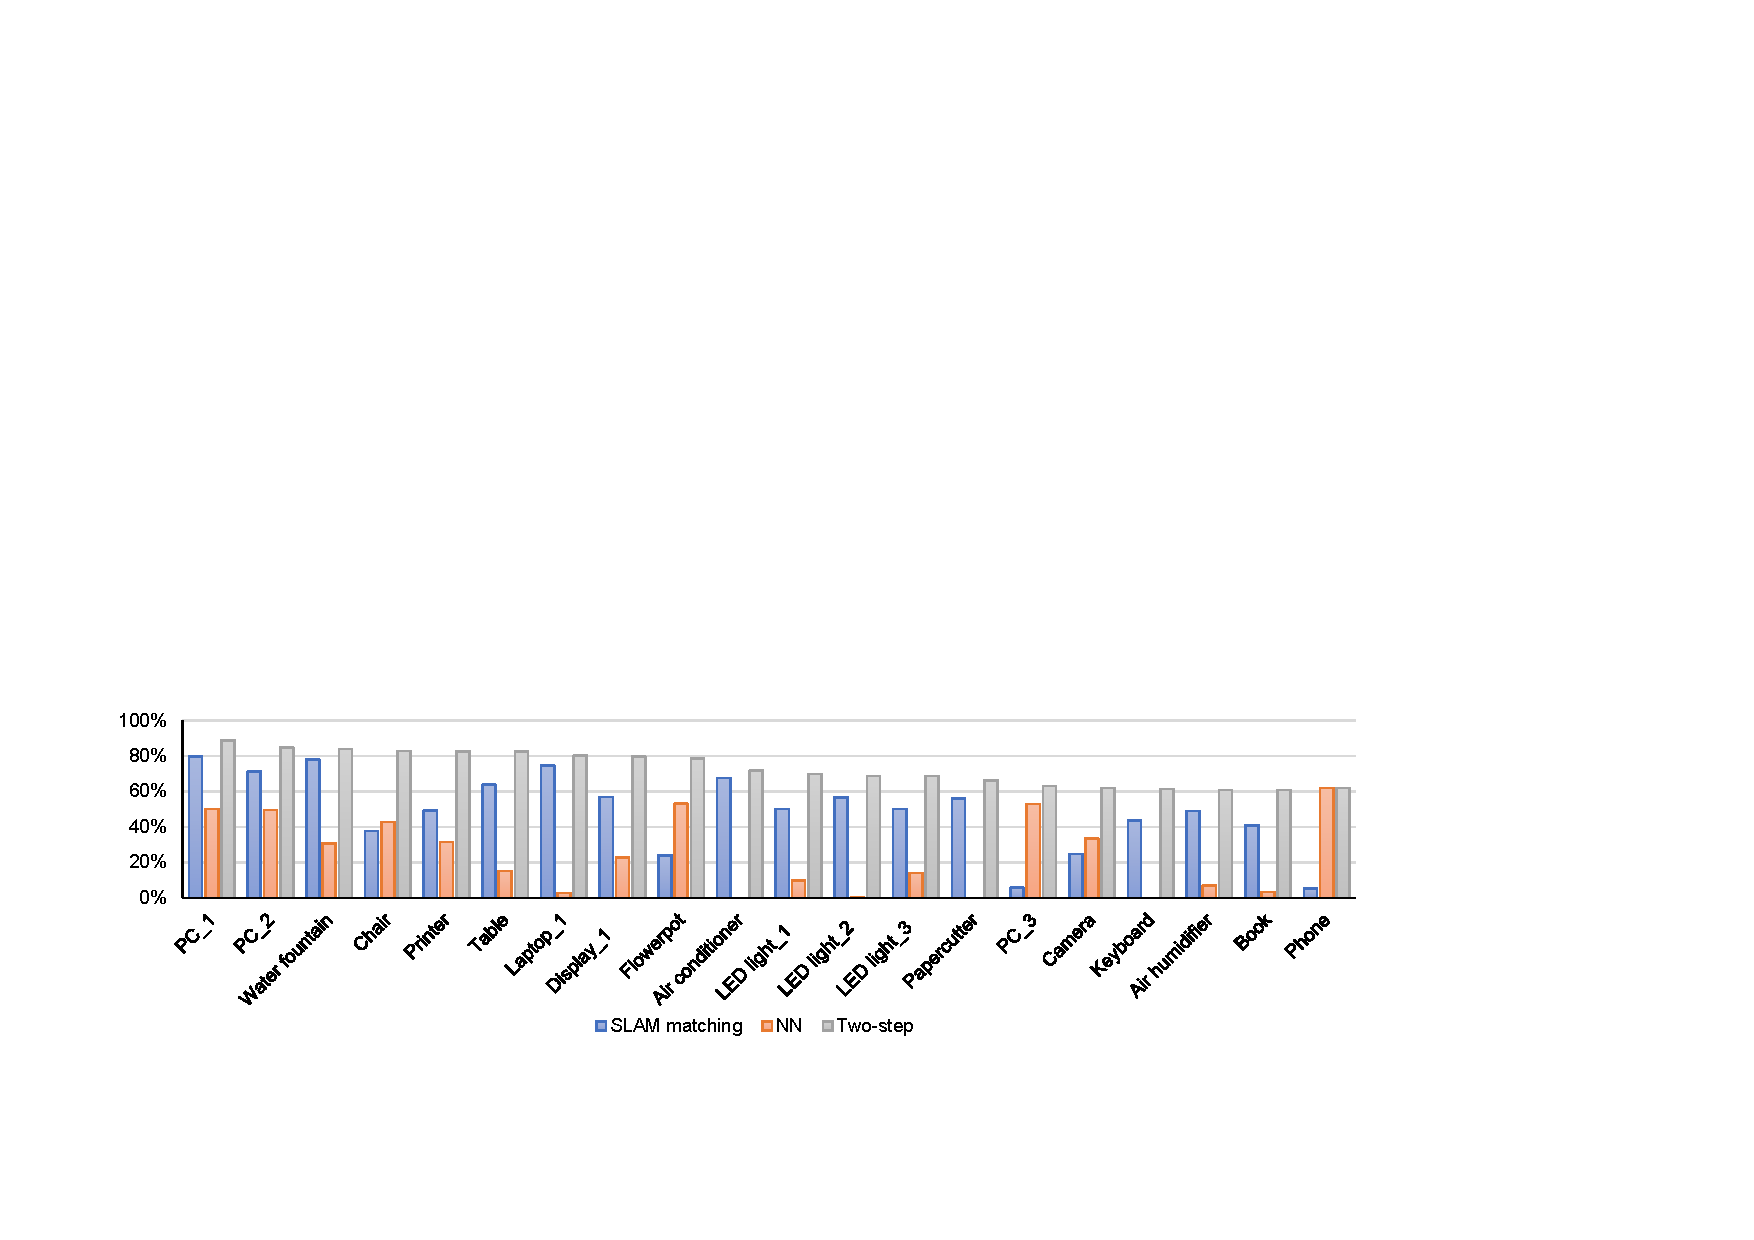
\includegraphics[width=0.95\linewidth]{ident-res}
	\caption{使用子图后目标检测准确率的改善}
	\label{fig:identification}
\end{figure*}

\textbf{VSLink的识别准确率}:
我们计算了VSLink的识别准确率,并将结果绘制在\autoref{fig:identification}中。我们可以看到,两阶段识别平均准确率达到72.7\%。对于基于SLAM匹配的方法,平均准确率为49.2\%,而对于只基于神经网络的方法,平均准确率为44.7\%。这两种方法互为补充,实现了多目标识别。在这里,我们没有针对这种情况对神经网络进行再训练,因为我们希望它是通用的,并且我们认为在使用专门的神经网络时它应该会表现出更好的性能。

我们认为漏检可分为两种情况。
一是我们在SLAM匹配和神经网络检测方面都失败了,所以我们需要考虑1)训练更好的神经网络,2)重建地图,让这个对象有更多的附着的地图点。
二是小物体无法被VSLink所捕捉。非常小的物体对于VSLink来说是极大的挑战,因为它们既没有较多特征点,也不容易被神经网络检测到。
我们希望通过神经网络的改进提高对小目标检测的能力,学术界对此正在进行研究,并且取得了一定进展。

\textbf{移动物体的识别}:
对于第四次/第五次视频,我们手动移动了六个对象,包括三个稳定的对象和三个可移动的对象。
对于稳定的对象,我们将它们移动了一小段距离(小于50厘米)。对于可移动的物体,我们将它们移动了很长的距离(超过2米)。
我们测试了VSLink是否可以重新识别移动的对象。
结果表明,该方法对稳定物体的识别准确率为83\%,对可移动物体的识别准确率为66\%。
由于我们依靠神经网络进行运动目标检测,如果需要提高可移动物体的识别率,需要我们采用更先进、更精确的网络。


\textbf{鲁棒性}:
我们通过五天的使用评估了VSLink的鲁棒性。在第四天和第五天,我们在环境中手动移动了一些对象。
实验结果显示,在最后一天,对象识别的准确率下降了10\%。我们分析了实验数据,发现基于SLAM匹配的识别在不同的光照条件或环境变化时出现了更多的未匹配点。这意味着我们需要随着时间的推移主动更新地图,否则地图会随时间流逝而逐渐失效。
而时间因素通常不会影响基于神经网络的检测的鲁棒性。

在我们的实现中,我们还没有实现地图实时更新的方法,但我们认为这是可行的。地图实时更新面临的挑战是主动更新地图点并对其进行标记,这需要执行实例分割神经网络,并且需要花费大量时间。
我们可以让我们的主线程,即两阶段对象识别过程,占用主要的计算资源。
地图更新线程以延后的方式执行。


\section{交互定制实验}

\begin{figure*}[htbp]
	\centering
	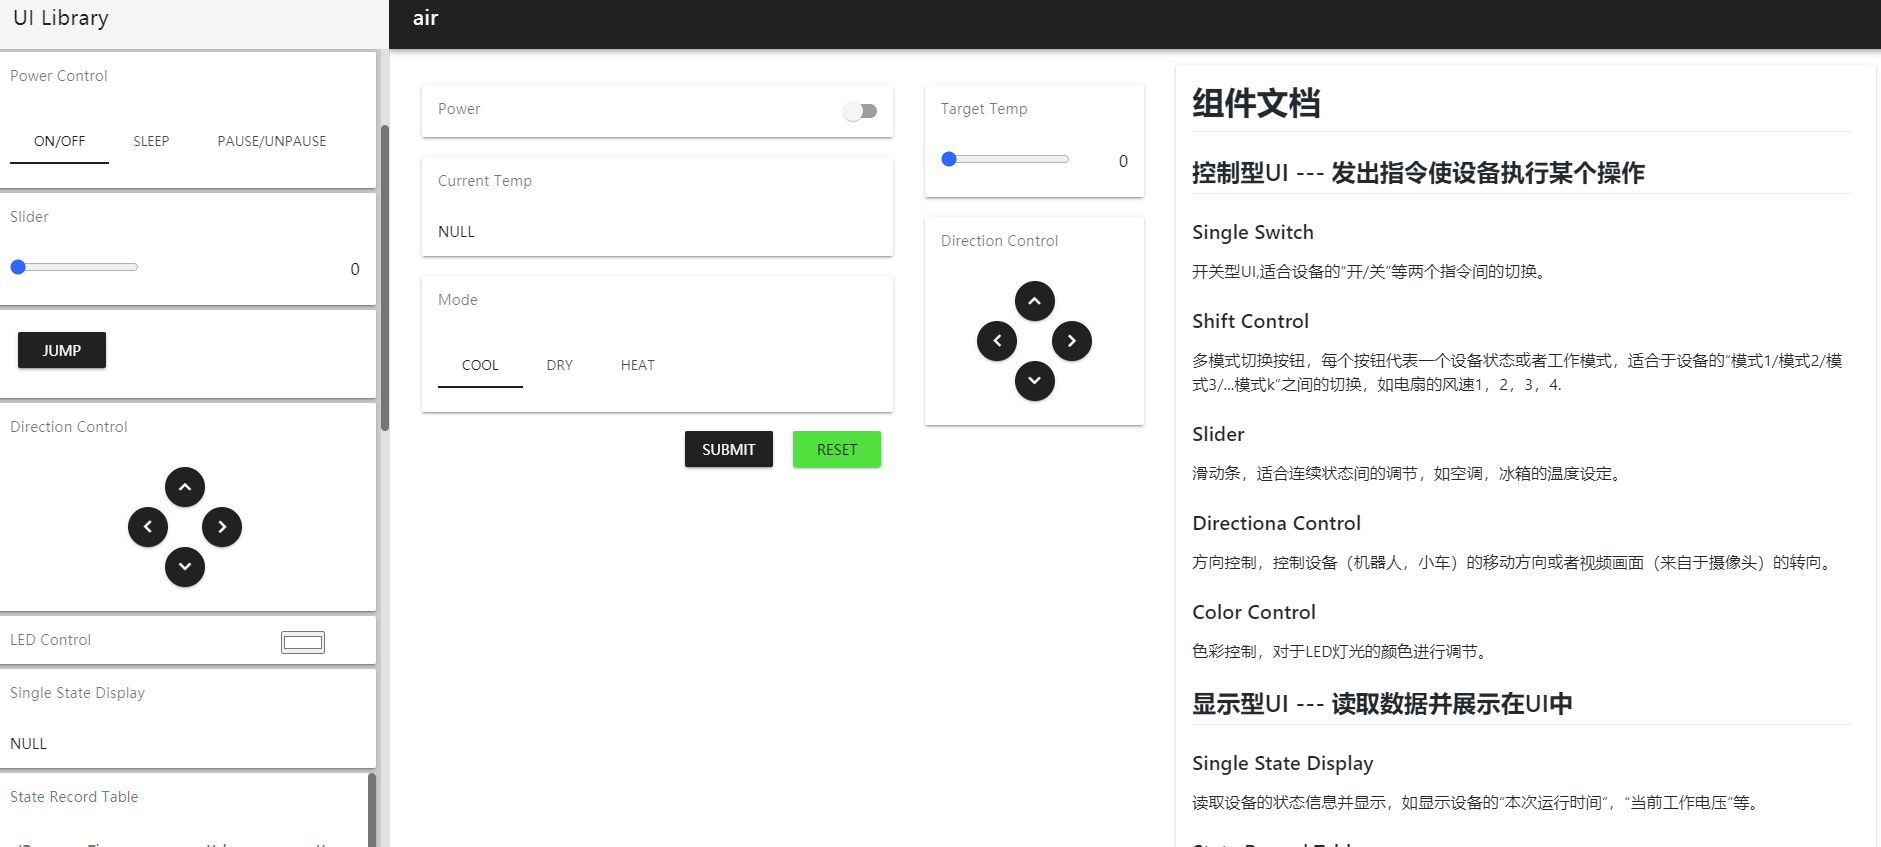
\includegraphics[width=0.95\linewidth]{UIdesign}
	\caption{UI定制页面}
	\label{fig:ui}
\end{figure*}

为了评估VSLink如何实现灵活的用户交互定制,我们进行了一项用户调研。在用户调研中,我们为参与者提供了一份详细的按步骤进行指导操作的用户手册,以指导他们使用VSLink设计由自己定制的UI。UI设计过程通过Web应用程序实现,如\autoref{fig:ui}中所示。图中的页面左边是UI库,中间是用于定制的画布,左边是UI的文档。

\textbf{用户调研中的开发者}: 
我们在学校招募了十名志愿者,其中包括五名博士生和五名硕士生。他们中的大多数人几乎都没有UI设计经验。我们要求每位志愿者通过VSLink实现两台设备的UI。我们在实验中收集了各个重要步骤的完成时间戳并分析了数据。


\textbf{量化结果}: 
首先,志愿者们被要求设计一个智能LED灯的UI,它有3个API。他们在按步骤编写的用户手册的指导下进行设计,结果表明志愿者们平均可以在五分钟内完成设计。第一个实验一般需要比正常流程更长的时间,因为志愿者需要首先学习如何使用VSLink和阅读UI文档之后才能开始正常使用。
接下来,志愿者们被要求设计一个智能风扇的UI,它有7个API,我们没有提供任何额外指导。这次设计的过程平均需要2分钟40秒。实验结果表明,在完成第一次实验后,后续的实验中志愿者们的设计速度大大提高。
最后,为了评估提供模板的情况下用户设计UI的速度,我们让志愿者使用VSLink提供的模板再次设计LED灯和智能风扇的UI。结果表明,以模板作为设计基础的情况下,志愿者完成LED灯和智能风扇的UI设计平均只需要31秒和1米28秒。

\textbf{志愿者反馈}:
为了获得志愿者的其他意见,我们询问了志愿者对时间成本、定制模板和页面美化的意见,获得了以下意见:
\begin{itemize}
  \item 所有志愿者都认为时间成本是可以接受的;
  \item 八名志愿者认为他们自己定制出来的UI比我们提供的模板更好,另外两人则认为两者没有大的区别;
  \item 一半的志愿者认为他们设计UI的网页还有进一步改进和美化的空间。
\end{itemize}



\section{案例验证}
演示VSLink在人机交互方面的能力。在这里,我们在\autoref{fig:cases}中展示了由VSLink开发的三个应用程序。第一个是智能会议室,我们将VSLink连接到会议室的设备,并设计相应的UI。用户可以通过VSLink控制门、投影仪、扬声器和空调。
二是植物养护。对于养植物的用户,我们设计了交互功能来记录浇水时间和浇水量,并记录重要日期,如开花日。
三是设备管理。对于实验室中的公共设备,我们记录并显示其元数据,如正式用户、当前用户、数据表等。此功能有助于管理大型设备。
我们要求10名志愿者评估VSLink的定制交互设计。
志愿者都是校园里的学生。
我们要求他们为随机选择的对象设计UI。
在实验中,他们平均需要两分钟即可完成设计。

\begin{figure}[htb]
	\centering
	\begin{subfigure}{.65\linewidth}
		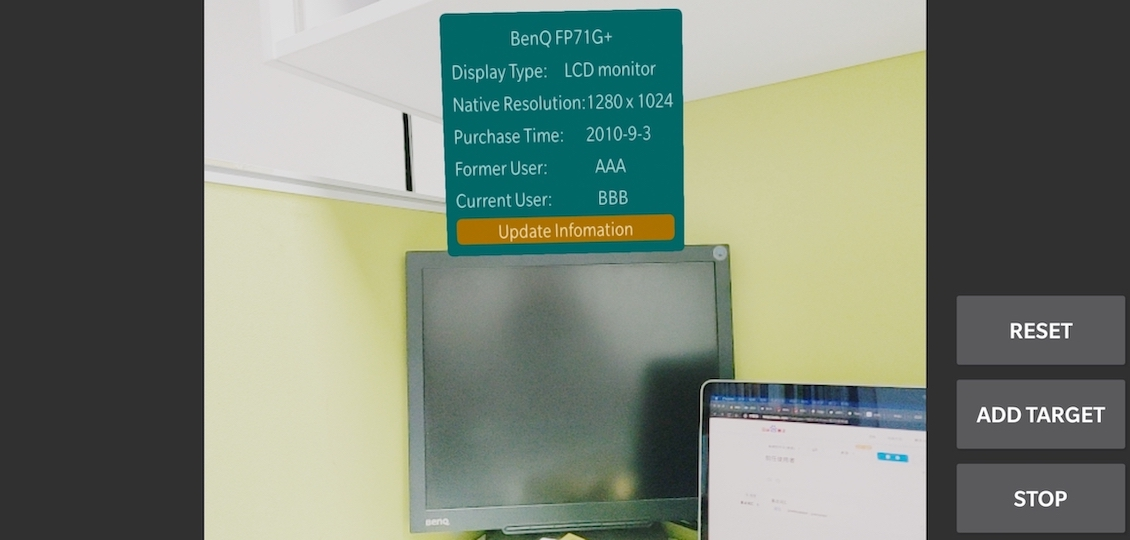
\includegraphics[width=1\linewidth]{case1}
		\caption{}
	\end{subfigure}
	%\hskip2em\
	%\centering
	\begin{subfigure}{.65\linewidth}
		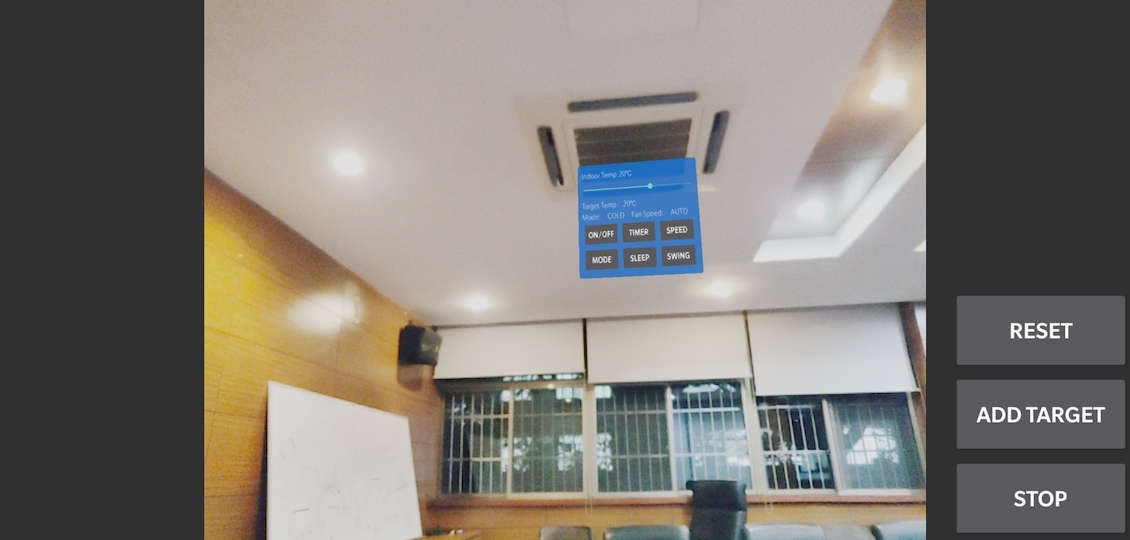
\includegraphics[width=1\linewidth]{case2}
		\caption{}
	\end{subfigure}
	\begin{subfigure}{.65\linewidth}
		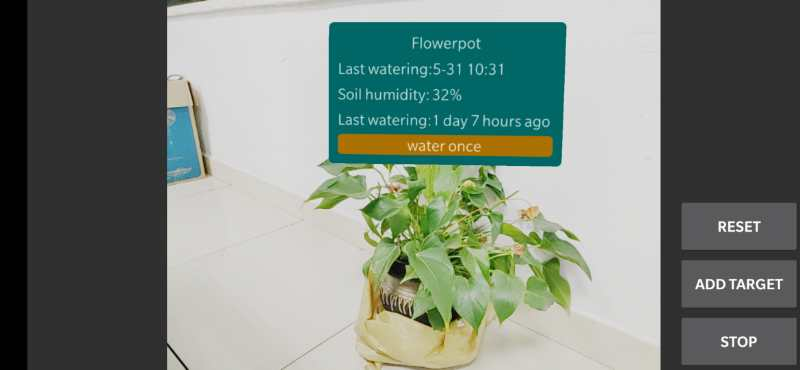
\includegraphics[width=1\linewidth]{case3}
		\caption{}
	\end{subfigure}
	\caption{三个VSLink实现的应用}\label{fig:cases}
\end{figure}




\chapter{总结}
\label{chap:sum}
在本文中,我们提出了VSLink,这是一种基于视觉技术的方法,用于实现与环境对象的快速和普适交互。
在VSLink中,我们利用视觉SLAM识别对象,并加速对象检测神经网络,使总的延迟小于33ms。VSLink还为用户提供了一个平台,以实现用户定制的交互,其中自定义UI是以无代码的方式开发的。
我们在包含多个要交互的对象的环境中评估了VSLink。结果表明,该算法在30fps的视频输入下具有良好的性能,目标识别率为{\acc}。

% \chapter{参考命令}
% \section{节标题}

% 我们可以用includegraphics来插入现有的jpg等格式的图片,
% 如\autoref{fig:zju-logo}所示。

% \begin{figure}[htbp]
%     \centering
%     \includegraphics[width=.3\linewidth]{logo/zju}
%     \caption{\label{fig:zju-logo}浙江大学LOGO}
% \end{figure}


% \subsection{小节标题}


% \par 如\autoref{tab:sample}所示,这是一张自动调节列宽的表格。

% \begin{table}[htbp]
%     \caption{\label{tab:sample}自动调节列宽的表格}
%     \begin{tabularx}{\linewidth}{c|X<{\centering}}
%         \hline
%         第一列 & 第二列 \\ \hline
%         xxx & xxx \\ \hline
%         xxx & xxx \\ \hline
%         xxx & xxx \\ \hline
%     \end{tabularx}
% \end{table}


% \par 如\autoref{equ:sample},这是一个公式

% \begin{equation}
%     \label{equ:sample}
%     A=\overbrace{(a+b+c)+\underbrace{i(d+e+f)}_{\text{虚数}}}^{\text{复数}}
% \end{equation}

% \chapter{另一章}

% \begin{figure}[htbp]
%     \centering
%     \includegraphics[width=.3\linewidth]{example-image-a}
%     \caption{\label{fig:fig-placeholder}图片占位符}
% \end{figure}